% -*- mode: latex; mode: reftex; mode: auto-fill; mode: flyspell; mode: yas/minor; coding: utf-8; tex-command: "pdflatex.sh" -*-

\documentclass[c,8pt]{beamer}

\usepackage[utf8]{inputenc}
\usepackage{overpic}
\usepackage{pgfplots}
\usepackage{xspace}
\usepackage{verbatimbox} % To insert verbatim inside \note

%%%%%%%%%%%%%%%%%%%%%%%%%%%%%%%%%%%%%%%%%%%%%%%%%%%%%%%%%%%%%%%%%%%%%%

%% \bibliographystyle{abbrvnat}
\bibliographystyle{includes/abbrvnatforbeamer}
\usepackage{multirow}

\usepackage{microtype}
\usepackage{amsmath}
\usepackage{amssymb}
\usepackage{dsfont}
\usepackage{verbatim}
\usepackage{upquote}
\usepackage{anyfontsize}
\usepackage[round]{natbib}
\usepackage{fancyvrb}
\usepackage{mathtools}
\usepackage{etex}
\usepackage{xparse}
\usepackage{xifthen}
%% \usepackage{BOONDOX-cal}

\def\theurl{\url{https://fleuret.org/dlc/}}
\def\theauthor{Fran\c cois Fleuret}
\def\coursetitle{Deep learning}

\makeatletter
\DeclareFontEncoding{LS1}{}{}
\DeclareFontSubstitution{LS1}{stix}{m}{n}
\DeclareMathAlphabet{\mathcal}{LS1}{stixscr}{m}{n}
\makeatother

\def\relu{\operatorname{ReLU}}
\def\softmax{\operatorname{softmax}}
\def\sigmoid{\operatorname{sigm}}
\def\sample{\operatorname{sample}}
\def\diag{\operatorname{diag}}
\def\sign{\operatorname{sign}}
\def\argmax{\operatornamewithlimits{argmax}}
\def\argmin{\operatornamewithlimits{argmin}}
\def\trace{\operatorname{Tr}}

% Olivier: I changed {\it #1} to \textit{#1} because there are
% different and does not mess up with serif/sansserif
%
% https://tex.stackexchange.com/questions/8053/is-there-a-difference-between-textit-and-itshape
\newcommand{\latin}[1]{\textit{#1}}
% \newcommand{\latin}[1]{{\it #1}}

\newcommand{\materialsurl}[1]{\url{https://fleuret.org/dlc/#1}}

\newcommand{\DATAVAR}{\mathbf{{\cal D}}}
\newcommand{\DATAVAL}{\mathbf{d}}
\newcommand{\BD}{\mathbf{D}}
\newcommand{\LL}{\mathcal{L}}
\newcommand{\Ll}{\mathcal{l}}
\newcommand{\RR}{\mathbb{R}}
\newcommand{\Lh}{\mathcal{h}}
\newcommand{\transpose}{^{\top}}

\newcommand{\dd}[2]{\frac{\partial {#1}}{\partial {#2}}}
%%\newcommand{\jacob}[2]{\left[ \dd{#1}{{#2}} \right]}
\newcommand{\gradient}[2]{\left[ \dd{#1}{{#2}} \right]}
%% \newcommand{\jacob}[2]{\mathbf{J}_{#1}}
\newcommand{\DD}[2]{\left[ \frac{\partial {#1}}{\partial {#2}} \right]}
\newcommand{\lbb}{\left[\!\!\left[}
\newcommand{\rbb}{\right]\!\!\right]}

\newcommand{\parname}[1]{{(#1)}}
\newcommand{\naming}[1]{{\text{(#1)}}}

%% \newcommand{\parname}[1]{{\vec{#1}}}
%% \newcommand{\parname}[1]{{\widetilde{#1}}}
%% \newcommand{\parname}[1]{{\tilde{#1}}}
%% \newcommand{\parname}[1]{{(#1)}}

%% \DeclareMathOperator*{\expect}{\mathds{E}}
%% \DeclareMathOperator*{\variance}{\mathds{V}}
%% \DeclareMathOperator*{\empexpect}{\hat{\mathds{E}}}
%% \DeclareMathOperator*{\mutinf}{\mathds{I}}
%% \DeclareMathOperator*{\empmutinf}{\hat{\mathds{I}}}
%% \DeclareMathOperator*{\entropy}{\mathds{H}}
%% \DeclareMathOperator*{\empentropy}{\hat{\mathds{H}}}

\def\given{\,\middle\vert\,}
\newcommand{\proba}{{P}}
\newcommand{\seq}{{S}}
%% \newcommand{\proba}{\mathds{P}}
\newcommand{\expect}{\mathds{E}}
\newcommand{\variance}{\mathds{V}}
\newcommand{\empexpect}{\hat{\mathds{E}}}
\newcommand{\mutinf}{\mathds{I}}
\newcommand{\empmutinf}{\hat{\mathds{I}}}
\newcommand{\entropy}{\mathds{H}}
\newcommand{\empentropy}{\hat{\mathds{H}}}
\newcommand{\ganG}{\mathbf{G}}
\newcommand{\ganD}{\mathbf{D}}
\newcommand{\ganF}{\mathbf{F}}

\newcommand{\dkl}{\mathds{D}_{\mathsf{KL}}}
\newcommand{\djs}{\mathds{D}_{\mathsf{JS}}}

\newcommand*{\vertbar}{\rule[-1ex]{0.5pt}{2.5ex}}
\newcommand*{\horzbar}{\rule[.5ex]{2.5ex}{0.5pt}}

\usepackage{xcolor}

%%%%%%%%%%%%%%%%%%%%%%%%%%%%%%%%%%%%%%%%%%%%%%%%%%%%%%%%%%%%%%%%%%%%%%
%% Colors

\definecolor{blue}{rgb}{0.0,0.0,0.55}
\definecolor{paleblue}{rgb}{0.50,0.50,1.00}
\definecolor{darkblue}{rgb}{0.10,0.10,0.70}

\definecolor{red}{rgb}{1.0,0.0,0.0}
\definecolor{palered}{rgb}{1.00,0.50,0.50}
\definecolor{darkred}{rgb}{0.75,0.0,0.0}

\definecolor{green}{rgb}{0.0,0.50,0.0}
\definecolor{palegreen}{rgb}{0.5,1.00,0.5}
\definecolor{darkgreen}{rgb}{0.0,0.5,0.0}

\definecolor{dimmed}{rgb}{0.8,0.8,0.8}

\definecolor{orange}{rgb}{1.0,0.6,0.0}
\definecolor{bluegray}{rgb}{0.1,0.2,0.7}

\newcommand{\blue}{\color{blue}}
\newcommand{\darkblue}{\color{darkblue}}
\newcommand{\paleblue}{\color{paleblue}}
\newcommand{\green}{\color{green}}
\newcommand{\darkgreen}{\color{darkgreen}}
\newcommand{\palegreen}{\color{palegreen}}
\newcommand{\red}{\color{red}}
\newcommand{\darkred}{\color{darkred}}
\newcommand{\palered}{\color{palered}}
\newcommand{\black}{\color{black}}

%%%%%%%%%%%%%%%%%%%%%%%%%%%%%%%%%%%%%%%%%%%%%%%%%%%%%%%%%%%%%%%%%%%%%%

\newcommand{\quotepaper}[2]{%
\begin{center}%
%
\begin{minipage}{0.95\textwidth}
``#2''
\end{minipage}%
%
\end{center}

\vspace*{-1ex}

\acksource{\citep{#1}}
}

%%%%%%%%%%%%%%%%%%%%%%%%%%%%%%%%%%%%%%%%%%%%%%%%%%%%%%%%%%%%%%%%%%%%%%

\newcommand{\quotesource}[2]{%
\begin{center}%
%
\begin{minipage}{0.95\textwidth}
``#2''
\end{minipage}%
%
\end{center}

\vspace*{-1ex}

\acksource{#1}
}

%%%%%%%%%%%%%%%%%%%%%%%%%%%%%%%%%%%%%%%%%%%%%%%%%%%%%%%%%%%%%%%%%%%%%%

\definecolor{codecolor}{rgb}{0.0,0.0,0.0}
\definecolor{codecolor2}{rgb}{0.0,0.0,0.0}

%% One keyword. The heavy magic to allow the percent symbol
%% \makeatletter
%% \newcommand{\kw}{\catcode`\%=12\@kw}
%% \DeclareRobustCommand{\@kw}[1]{{{\color{codecolor}\tt \detokenize{#1}}\catcode`\%=14}{}}
%% \makeatother
\DeclareRobustCommand{\kw}[1]{{\color{codecolor}\tt \detokenize{#1}}}

%% Inline piece of code

\DefineVerbatimEnvironment{rawsrc}{BVerbatim}{fontsize=\small,baselinestretch=1.0,formatcom=\color{codecolor}}

%% Sub-part of a file

\ifnum\pdfshellescape=1
\NewDocumentCommand{\rawsrcexcerpt}{mmmO{}O{1}}{%
  \BVerbatimInput[fontsize=\small,baselinestretch=1.0,formatcom=\color{codecolor},#4]{|"< #1 awk '/#2/{flag=1;next}/#3/{flag=0}flag {print substr($0, #5)}' | grep -v HIDE_IN_SLIDE"}%
}
\else
\NewDocumentCommand{\rawsrcexcerpt}{mmmO{}O{1}}{%
  {\color{darkred} \tt Source snippet omitted because shell escape is disabled.}%
}
\fi

%%%%%%%%%%%%%%%%%%%%%%%%%%%%%%%%%%%%%%%%%%%%%%%%%%%%%%%%%%%%%%%%%%%%%%

\newenvironment{warning}{%
\raisebox{-8pt}{%
\begin{tikzpicture}[scale=0.6]
\node at (0, 0) {\huge\textrm{\textbf{!}}};
\draw[rounded corners=1pt,line width=1.5pt,darkred] (-0.6, -0.47) -- ++(1.2, 0) -- ++(-0.6, 1.2) -- cycle;
\end{tikzpicture}%
}%
%% {\darkred \huge {\fontencoding{U}\fontfamily{futs}\selectfont\char 66\relax}}%
%
\hspace*{0.75em}%
%
\begin{minipage}{0.9\textwidth}
}{%
\end{minipage}%
}

%%%%%%%%%%%%%%%%%%%%%%%%%%%%%%%%%%%%%%%%%%%%%%%%%%%%%%%%%%%%%%%%%%%%%%

\newcommand{\fixedheightbox}[2]{%
   \sbox{0}{\parbox{\textwidth}{#2}}
    \ifdim\dimexpr\ht0+\dp0<#1
    \dp0\dimexpr#1-\ht0\fi
    \usebox{0}%
}

\makeatletter
\newcommand{\smallerthantiny}{\@setfontsize{\smallerthantiny}{4pt}{5pt}}
\makeatother

%%%%%%%%%%%%%%%%%%%%%%%%%%%%%%%%%%%%%%%%%%%%%%%%%%%%%%%%%%%%%%%%%%%%%%
%% The \draft command

\newcounter{nbdrafts}
\setcounter{nbdrafts}{0}
\makeatletter
\newcommand{\checknbdrafts}{
\ifnum \thenbdrafts > 0
\@latex@warning@no@line{**********************************************************************}
\@latex@warning@no@line{* The document contains \thenbdrafts \space draft note(s)}
\@latex@warning@no@line{**********************************************************************}
\fi}
\newcommand{\draft}[1]{\addtocounter{nbdrafts}{1}{\color{red} #1}}
\makeatother

\newcommand{\vstretch}{\vspace*{\stretch{1}}}
\newcommand{\hstretch}{\hspace*{\stretch{1}}}

%%%%%%%%%%%%%%%%%%%%%%%%%%%%%%%%%%%%%%%%%%%%%%%%%%%%%%%%%%%%%%%%%%%%%%
% Across files references, e.g. \dlclabel{autograd} in the slide file
% about autograd, and \dlcref{autograd} where we want to refer to it

\newcommand{\dlclabel}[1]{%
\newwrite\file
\immediate\openout\file=#1.dlcref
%% \immediate\write\file{\dlclecturenumber.\dlcdecknumber.\,``\detokenize\expandafter{\dlcdecktitle}''}
%\immediate\write\file{\dlclecturenumber.\dlcdecknumber.\detokenize\expandafter{\,``\dlcdecktitle''}}
\immediate\write\file{\dlclecturenumber.\dlcdecknumber. ``\dlcdecktitle''}
\immediate\closeout\file
}

\newcommand{\dlcref}[1]{%
\InputIfFileExists{#1.dlcref}{}{[dlcref #1 undefined]}\unskip
%\@input{#1.dlcref}\unskip
}%

%%%%%%%%%%%%%%%%%%%%%%%%%%%%%%%%%%%%%%%%%%%%%%%%%%%%%%%%%%%%%%%%%%%%%%

% To include a .pdf image which itself includes a raster image
% relative to itself
%
% https://tex.stackexchange.com/a/282110
\newcommand\inputpgf[2]{{
\let\pgfimageWithoutPath\pgfimage
\renewcommand{\pgfimage}[2][]{\pgfimageWithoutPath[##1]{#1/##2}}
\input{#1/#2}
}}


\usepackage{tikz}

\usetikzlibrary{positioning,fit,backgrounds}
\usetikzlibrary{arrows.meta,decorations.pathreplacing}
\usetikzlibrary{calc}
\usetikzlibrary{shapes,calc,intersections}
\usetikzlibrary{patterns}
%% \usetikzlibrary{shapes.multipart}

\usetikzlibrary{arrows}
%% \tikzset{>=angle 90}

\definecolor{nn-data}   {rgb}{0.90, 0.95, 1.00}
\definecolor{nn-param}  {rgb}{1.00, 0.90, 0.50}
\definecolor{nn-process}{rgb}{0.80, 1.00, 0.80}

\tikzset{
  pics/box/.style args={#1/#2/#3/#4/#5/#6}{
    code={
      \pgfmathsetmacro{\slant}{0.35}
      \pgfmathsetmacro{\width}{#1}
      \pgfmathsetmacro{\height}{#2}
      \pgfmathsetmacro{\thickness}{#3}
      \pgfmathsetmacro{\lwidth}{#4}
      \pgfmathsetmacro{\lheight}{#5}
      \pgfmathsetmacro{\lthickness}{#6}
      \pgfmathsetmacro{\labelgap}{0.15}

      \pgfmathsetmacro{\centerx}{0}
      \pgfmathsetmacro{\centery}{\height * 0.5 + \width * 0.5 * \slant}

      % Filled body

      \draw[fill] ( - \centerx, - \centery)
      -- ++(0.0, \height)
      -- ++(\slant * 0.5 * \width, 0.5 * \width)
      -- ++(\thickness, 0.0)
      -- ++(0, -\height)
      -- ++(- \slant * 0.5 * \width, -0.5 * \width)
      -- ++(-\thickness, 0)
      ;

      % Additional edges

      \draw  ( - \centerx, - \centery) ++(0.0, \height)
      -- ++(\thickness, 0.0) -- ++(\slant * 0.5 * \width, 0.5 * \width)
      ;

      \draw  ( - \centerx, - \centery) ++(\thickness, \height)
      -- ++(0.0, -\height)
      ;

      % Axis length labels

      \ifthenelse
      {\equal{\lwidth}{}}{}
      {
        \draw[<->]  ( - \centerx, - \centery) ++(0.0, \height) ++(-\labelgap * .7071, \labelgap * .7071)
        -- ++(\slant * 0.5 * \width, 0.5 * \width) node[midway, above left] {\scriptsize \lwidth};
      }

      \ifthenelse
      {\equal{\lheight}{}}{}
      {
        \draw[<->]  ( - \centerx, - \centery) ++(-\labelgap, 0.0)
        -- ++(0.0, \height) node[midway, left] {\scriptsize \lheight};
      }

      \ifthenelse
      {\equal{\lthickness}{}}{}
      {
        \draw[<->]  ( - \centerx, - \centery) ++(0.0, -\labelgap)
        -- ++(\thickness, 0.0) node[midway, below] {\scriptsize \lthickness};
      }

      % Anchor points

      \coordinate (-center) at (\thickness + \slant * 0.25 * \width, 0.0);

      \coordinate (-follow-tight) at (\thickness + 0.2, 0.0);

      \coordinate (-follow-close) at (\thickness + \slant * 0.5 * \width, 0.0);

      \coordinate (-follow) at (\thickness + \slant * 0.2 * \width + 1.0, 0.0);

      \coordinate (-above-back)  at (-\centerx + \slant * 0.5 * \width + \thickness * 0.5, \height - \centery + 0.5 * \width + 0.3);

      \coordinate (-above)  at (-\centerx + \thickness * 0.5, \height - \centery + 0.5 * \width + 0.3);

      \coordinate (-below)  at (-\centerx + \thickness * 0.5, -\centery - 0.5);
    }
  },
  pics/box/.default=0.5/1/1/1/1/1
}

%%%%%%%%%%%%%%%%%%%%%%%%%%%%%%%%%%%%%%%%%%%%%%%%%%%%%%%%%%%%%%%%%%%%%%

%% \newcommand{\intint}[1]{[\![#1]\!]}
\newcommand{\intint}[1]{[\![#1]\!]}

\newcommand{\cube}[6]{
    \draw[#1,#2] #3 -- ++#4 -- ++#5 -- ++#6 -- ++($(0, 0) - #4$) -- ++($(0, 0) - #5$) -- ++($(0, 0) - #6$);
    \draw[#1] #3 ++#4 -- ++#6 -- ++#5;
    \draw[#1] #3 ++#6 -- ++#4;
}

%%%%%%%%%%%%%%%%%%%%%%%%%%%%%%%%%%%%%%%%%%%%%%%%%%%%%%%%%%%%%%%%%%%%%%

\newcommand{\oneconv}[3]{
  \uncover<#1>{
    \cube{draw=black,thick}{fill=black!15}{#3}{(0, 1)}{(0.4, 0.8)}{(1, 0)}
  }

  \uncover<#1-#2>{
    \cube{draw=green,thick}{fill=white}{#3 ++(7.4, 0.4)}{(0, 0.6)}{(0.2, 0.4)}{(0.33333, 0)}
  }
}

\newcommand{\onepool}[3]{
  \uncover<#1>{
    \cube{draw=black,thick}{fill=black!15}{#3}{(0, 1)}{(0.4, 0.8)}{(1, 0)}
  }

  \uncover<#1-#2>{
    \cube{draw=green,thick}{fill=white}{#3 ++(7.4, 0.4)}{(0, 0.6)}{(0.2, 0.4)}{(0.33333, 0)}
  }
}

%%%%%%%%%%%%%%%%%%%%%%%%%%%%%%%%%%%%%%%%%%%%%%%%%%%%%%%%%%%%%%%%%%%%%%

\newcommand{\drawvector}[1]{
%% \raisebox{0.75cm}{\Large $\Bigg($}
\begin{tikzpicture}[scale=0.2]
  \draw[draw=none] (0, -4) -- (0, 4);
  \edef\xdraw{0}
  \draw[black!20,thin] (0, -0.2) -- ++(0, 0.4);
  \foreach \y in { #1 }{
    \pgfmathparse{\xdraw+1}
    \xdef\xdraw{\pgfmathresult}
    \draw[black!20,thin] (\xdraw, -0.2) -- ++(0, 0.4);
  }
  \draw[black!20,thin] (-0.1, 0) -- (\xdraw, 0) ++(0.1, 0);
  \edef\xdraw{0}
  \foreach \y in { #1 }{
    \draw[] (\xdraw, 0) -- ++(0, \y) -- ++(1.0, 0.0) -- ++(0, -\y);
    %% \draw[] (\xdraw, \y) -- ++(0.05, 0) -- ++(0.9, 0.0);
    %% \draw[thick] (\xdraw,\y) +(0.05, 0) -- ++(0.9, 0.0);
    \pgfmathparse{\xdraw+1}
    \xdef\xdraw{\pgfmathresult}
  }
\end{tikzpicture}%
%% \raisebox{0.75cm}{\Large $\Bigg)$}
}

%%%%%%%%%%%%%%%%%%%%%%%%%%%%%%%%%%%%%%%%%%%%%%%%%%%%%%%%%%%%%%%%%%%%%%

%%%%%%%%%%%%%%%%%%%%%%%%%%%%%%%%%%%%%%%%%%%%%%%%%%%%%%%%%%%%%%%%%%%%%%
% A command to illustrate the convolutional layer output size

\newcommand{\convscheme}[4]{
\begin{tikzpicture}[scale=0.15]
\draw (0, 0) -- (#1, 0);
\draw[<->] (0, 1.75) -- ++(#1, 0) node[midway,above] {$#1$};

\draw[fill=green!25] (#1, 0.00) ++(-#2, 0.0) rectangle ++(#2, 1.0);

\foreach \x in { 1,...,#1 }
  \draw[thin] (\x, 0.0) ++(-1, 0) rectangle ++(1, 1);

\draw[] (0, 0.00) ++(0, -0.5) -- ++({#3*(#4-1)+1}, 0.0) node[midway,below] {$\times #4$};

\foreach \x in { 1,...,#4 }
  \draw[fill=black] ({#3*(\x-1)}, 0.5) ++(0.5, 0) circle(4pt);
\end{tikzpicture}
}

\newcommand{\convtransposescheme}[4]{
\begin{tikzpicture}[scale=0.15]
\draw (0, 0) -- (#1, 0);

\draw[fill=green!25] (#1, 0.00) ++(-#2, 0.0) rectangle ++(#2, 1.0);

\foreach \x in { 1,...,#1 }
  \draw[thin] (\x, 0.0) ++(-1, 0) rectangle ++(1, 1);

\draw[] (0, 0.00) ++(0, 1.5) -- ++({#3*(#4-1)+1}, 0.0) node[midway,above] {$\times #4$};
%% \draw[<->] (#1, 0.00) ++(-#2, -0.75) -- ++(#2, 0.0) node[midway,below] {$#2$};
\draw[<->] (0, -0.75) -- ++(#1, 0.00) node[midway,below] {$#1$};

\foreach \x in { 1,...,#4 }
  \draw[fill=black] ({#3*(\x-1)}, 0.5) ++(0.5, 0) circle(4pt);
\end{tikzpicture}
}

%%%%%%%%%%%%%%%%%%%%%%%%%%%%%%%%%%%%%%%%%%%%%%%%%%%%%%%%%%%%%%%%%%%%%%

\tikzset{>={Straight Barb[angle'=80,scale=1.1]}}

\tikzset{
  value/.style    ={ font=\scriptsize, rectangle, draw=black!50, fill=white,   thick,
                     inner sep=3pt, inner xsep=2pt, minimum size=10pt, minimum height=20pt },
  parameter/.style={ font=\scriptsize, rectangle, draw=black!50, fill=blue!15, thick,
                     inner sep=0pt, inner xsep=2pt, minimum size=10pt, minimum height=20pt },
  operation/.style={ font=\scriptsize, rectangle,    draw=black!50, fill=green!30, thick,
                     inner sep=3pt, minimum size=10pt, minimum height=20pt },
  flow/.style={->,shorten <= 1pt,shorten >= 1pt, draw=black!50, thick},
%
  f2f/.style={draw=black!50, thick},
  v2f/.style={{Bar[width=1.5mm]}-,shorten <= 0.75pt,draw=black!50, thick},
  f2v/.style={->,shorten >= 0.75pt,draw=black!50, thick},
  v2v/.style={{Bar[width=1.5mm]}->,shorten <= 0.75pt,shorten >= 0.5pt,draw=black!50, thick},
%
%
  df2f/.style={draw=black, thick},
  dv2f/.style={{Bar[width=1.5mm]}-,shorten <= 0.75pt,draw=black, thick},
  df2v/.style={->,shorten >= 0.75pt,draw=black, thick},
  dv2v/.style={{Bar[width=1.5mm]}->,shorten <= 0.75pt,shorten >= 0.5pt,draw=black, thick},
%
  differential/.style    ={ font=\small, rectangle, draw=black!50,               thick,
                     inner sep=3pt, inner xsep=2pt, minimum size=10pt, minimum height=20pt, fill=yellow!80 },
  dflow/.style={->,shorten <= 1pt,shorten >= 1pt, draw=black, thick}
}

\newcommand{\nophone}{
\begin{tikzpicture}

\draw[fill=black] (0, 0) to (0, 7) to [out=6,in=174] (4, 7) to (4, 0) to [out=186,in=354] (0, 0);

\draw[fill=white] (0.2, 0.75) rectangle (3.8, 6.35);
\draw[fill=white] (2, 0.27) circle (0.2);
\draw[fill=white] (1, 6.7) circle (0.1);

\draw[line width=33pt,color=white] (2, 3.5) circle (5cm);
\draw[line width=33pt,color=white] (2, 3.5) ++(-3.3, -3.3) -- ++(6.6, 6.6);
\draw[line width=23pt,color=red] (2, 3.5) circle (5cm);
\draw[line width=23pt,color=red] (2, 3.5) ++(-3.3, -3.3) -- ++(6.6, 6.6);

\end{tikzpicture}
}

%\input{includes/source-highlight}

\pgfplotsset{compat=1.11}

%%%%%%%%%%%%%%%%%%%%%%%%%%%%%%%%%%%%%%%%%%%%%%%%%%%%%%%%%%%%%%%%%%%%%%
%% The witharrows mess due to my old Debian

\usepackage{witharrows} % To make explanatory arrows between equation lines

%% \usepackage{environ}
%% \NewEnviron{DispWithArrows*}{%
%% \begin{align}
%% \BODY
%% \end{align}
%% }
%% \newcommand{\Arrow}[1]{}

%%%%%%%%%%%%%%%%%%%%%%%%%%%%%%%%%%%%%%%%%%%%%%%%%%%%%%%%%%%%%%%%%%%%%%
%% Do not skip frame numbers
\usepackage{etoolbox}
\makeatletter
\pretocmd{\beamer@@@@frame}{\alt<#1>{}{\beamer@noframenumberingtrue}}{}{}
\makeatother
%%%%%%%%%%%%%%%%%%%%%%%%%%%%%%%%%%%%%%%%%%%%%%%%%%%%%%%%%%%%%%%%%%%%%%

%%%%%%%%%%%%%%%%%%%%%%%%%%%%%%%%%%%%%%%%%%%%%%%%%%%%%%%%%%%%%%%%%%%%%%
% To make an index
\newenvironment{theindex}{}{}
\usepackage{imakeidx}
\usepackage{fp}

\makeatletter
% Global redefinition of indexentry to use section, then page
\newcounter{tmpcounter}
\renewcommand{\imki@wrindexentrysplit}[3]{%
  %%%%%%%%%%%%%%%%%%%%%%%%%%%%%%%%%%%%%%%%%%%%%%%%%%%
  % To make the items easily sortable (integers) without redefining too
  % much xindy and co. an index is referenced with:
  % 13002007 : lecture 13, course 2, frame 7
  % 1000000 * lecture + 1000 * deck + frame
  %%%%%%%%%%%%%%%%%%%%%%%%%%%%%%%%%%%%%%%%%%%%%%%%%%%
  % End all following lines with '%' otherwise,
  % an extra space is generated by \index
  %%%%%%%%%%%%%%%%%%%%%%%%%%%%%%%%%%%%%%%%%%%%%%%%%%%
  \setcounter{tmpcounter}{\dlclecturenumber}%
  \ifnum \thetmpcounter > 999%
  \PackageError{dlc}{Lecture number (\dlclecturenumber) should be < 1000 for index encoding}{}%
  \fi%
  \setcounter{tmpcounter}{\dlcdecknumber}%
  \ifnum \thetmpcounter > 999%
  \PackageError{dlc}{Deck number (\dlcdecknumber) should be < 1000 for index encoding}{}%
  \fi%
  \FPeval{\indexid}{clip(1000000*\dlclecturenumber+1000*\dlcdecknumber+\insertframenumber)}%
  % \expandafter\protected@write\csname#1@idxfile\endcsname{}{\string\indexentry{#2}{\lecturenumber.\coursenumber:\insertframenumber}}%
  \expandafter\protected@write\csname#1@idxfile\endcsname{}{\string\indexentry{#2}{\indexid}}%
}%
\makeatother
%%%%%%%%%%%%%%%%%%%%%%%%%%%%%%%%%%%%%%%%%%%%%%%%%%%%%%%%%%%%%%%%%%%%%%

\makeindex

\let\oldindex\index % save old definition to prevent recursion
\renewcommand*\index[1]{\oldindex{#1|formatsliderange}}
% \renewcommand*\index[1]{\oldindex{#1|formatsliderange}\ignorespaces}
%%%%%%%%%%%%%%%%%%%%%%%%%%%%%%%%%%%%%%%%%%%%%%%%%%%%%%%%%%%%%%%%%%%%%%


% %%~~~~~~~~~~~~~~~~~~~~~~~~~~~~~~~~~~~~~~~~~~~~~~~~~~~~
% \mode<handout>{
%   \usepackage{pgfpages}
%   %% \pgfpagesuselayout{16 on 1}[a4paper,border shrink=0mm,landscape]
%   %% \pgfpageslogicalpageoptions{1}{border code=\pgfusepath{stroke}}
%   %% \pgfpageslogicalpageoptions{2}{border code=\pgfusepath{stroke}}
%   %% \pgfpageslogicalpageoptions{3}{border code=\pgfusepath{stroke}}
%   %% \pgfpageslogicalpageoptions{4}{border code=\pgfusepath{stroke}}
%   \pgfpagesuselayout{2 on 1}[a4paper,border shrink=4mm]
% }
% %% \setbeamercovered{transparent}
% %%~~~~~~~~~~~~~~~~~~~~~~~~~~~~~~~~~~~~~~~~~~~~~~~~~~~~

%%~~~~~~~~~~~~~~~~~~~~~~~~~~~~~~~~~~~~~~~~~~~~~~~~~~~
\usepackage{makecell}
%% To get handout on top of A4 page and not below, and to handle the
%% fact that some slides don't have notes.

\usepackage{ragged2e}  % justify text

\mode<handout>{
  % \setbeamercolor{background canvas}{bg=gray!10} % Olivier: debug handout
  \usepackage{pgfpages}
  %% \pgfpagesuselayout{16 on 1}[a4paper,border shrink=0mm,landscape]
  %% \pgfpageslogicalpageoptions{1}{border code=\pgfusepath{stroke}}
  %% \pgfpageslogicalpageoptions{2}{border code=\pgfusepath{stroke}}
  %% \pgfpageslogicalpageoptions{3}{border code=\pgfusepath{stroke}}
  %% \pgfpageslogicalpageoptions{4}{border code=\pgfusepath{stroke}}
  \pgfpagesuselayout{2 on 1}[a4paper,border shrink=3mm]

  \ifdefined\withoutnotes
    \ifdefined\withnotes
      \setbeameroption{show notes}
    \fi
  \else
    \setbeameroption{show notes}
    %% \pgfpageslogicalpageoptions{1}{border code=\pgfusepath{stroke}}
  \fi

  \setbeamertemplate{note page}{%

    \insertnote
  }
}
%%~~~~~~~~~~~~~~~~~~~~~~~~~~~~~~~~~~~~~~~~~~~~~~~~~~~

\catcode`\%=12
\newcommand\percentsymbol{%}
\catcode`\%=14

\def\closingmessage{The End}

%% \def\theauthor{Undefined author} % Author
%% \def\theurl{https://fleuret.org/dlc/}
%% \def\coursetitle{Undefined title}

\def\dlcdecktitle{Undefined subtitle}
%\def\coursenumber{}
\def\dlclecturenumber{} % for index
\def\dlcdecknumber{} % for index \lecturenb.\coursenb

%% \def\draftwarning{{\small \bf Draft, do not distribute}}
\def\draftwarning{}
%% \def\thedate{\scriptsize [version of: \today]}
\ifnum\pdfshellescape=1
%% \def\thedate{\small \input{|"date --utc -r \jobname.tex"}}
\def\thedate{\small \input{|"date +'\percentsymbol b \percentsymbol e, \percentsymbol Y' -r \jobname.tex"}}
\else
\def\thedate{\small Shell escape disabled}
\fi

\setlength{\parindent}{0cm}
\setlength{\parskip}{3ex}

\newcommand{\MM}{\mathcal M}
\newcommand{\TT}{\mathcal T}
%% \newcommand{\MM}{\mathscr M}
%% \newcommand{\TT}{\mathscr T}

\newcommand{\RD}{\mathbb{R}^D}
\newcommand{\st}{\,\text{s.t.}\,}

%% \usepackage{ebgaramond-maths}
%% \usepackage[T1]{fontenc}

%% \usepackage[round]{natbib}
%% \usepackage{natbib}
%% \bibliographystyle{abbrvnat}
%% \setcitestyle{authoryear,open={((},close={))}}

\usepackage{calc}

%% \usepackage{biblatex}
%% \AtEveryBibitem{%
  %% \clearfield{url}%
%% }

\newcommand{\mathand}{ \ \text{and} \ }

%% \tikzset{
  %% value/.style    ={ font=\small, rectangle, draw=black!50,               thick,
                     %% inner sep=0pt, inner xsep=2pt, minimum size=10pt },
  %% parameter/.style={ font=\small, rectangle, draw=black!50, fill=blue!30, thick,
                     %% inner sep=0pt, inner xsep=2pt, minimum size=10pt },
  %% operation/.style={ font=\scriptsize, circle,    draw=black!50, fill=blue!30, thick,
                     %% inner sep=0pt, minimum size=10pt },
  %% flow/.style={->,shorten <= 1pt,shorten >= 1pt, draw=black!50, thick}
%% }

%%%%%%%%%%%%%%%%%%%%%%%%%%%%%%%%%%%%%%%%%%%%%%%%%%%%%%%%%%%%%%%%%%%%%%
%% Font Open Sans light

%% \usepackage[default]{opensans}
%% \usepackage{cmbright}

%% \renewcommand{\familydefault}{fos}
%% \renewcommand{\seriesdefault}{l}
%% \renewcommand{\bfdefault}{sb}

%%%%%%%%%%%%%%%%%%%%%%%%%%%%%%%%%%%%%%%%%%%%%%%%%%%%%%%%%%%%%%%%%%%%%%
%% Colors

%% \mode<beamer>{
%% \setbeamercolor{math text}{fg=green}
\setbeamercolor{math text}{fg=bluegray}
\setbeamercolor{local structure}{fg=blue}
\definecolor{codecolor}{rgb}{0.0,0.4,0.5}%
\definecolor{codecolor2}{rgb}{0.0,0.7,0.0}%
%% }

%% \mode<handout>{
%% \setbeamercolor{math text}{fg=black}
%% \setbeamercolor{local structure}{fg=black}
%% }

%%%%%%%%%%%%%%%%%%%%%%%%%%%%%%%%%%%%%%%%%%%%%%%%%%%%%%%%%%%%%%%%%%%%%%
%% Remove the navigation bar, define the frame titles and footline

\newcommand{\titleemph}{}

\makeatletter
\define@key{beamerframe}{c}[true]{% centered
  \beamer@frametopskip=1em plus 1fill\relax%
  %% \beamer@frametopskip=0pt plus 1fill\relax%
  \beamer@framebottomskip=0pt plus 1fill\relax%
  \beamer@frametopskipautobreak=0pt plus .4\paperheight\relax%
  \beamer@framebottomskipautobreak=0pt plus .6\paperheight\relax%
  \def\beamer@initfirstlineunskip{}%
}
\makeatother

\setbeamertemplate{navigation symbols}{}
%% \setbeamersize{text margin left=2em,text margin right=2em}
\setbeamersize{text margin left=5em,text margin right=5em}
\setbeamertemplate{itemize item}{\raisebox{0.15ex}{\tiny \ensuremath{\black \bullet}}}
\setbeamertemplate{itemize subitem}{\raisebox{0.15ex}{\tiny \ensuremath{\black \bullet}}}
\setbeamerfont{frametitle}{size=\normalsize}

\setbeamercolor{normal text in math text}{fg=black}

%% \setlength{\textheight}{10cm}

\ifdefined\overrideframetitle\setbeamertemplate{frametitle}{\overrideframetitle}%
\else
\setbeamertemplate{frametitle}{
  \hskip-1.5em\usebeamerfont{frametitle}\titleemph{\insertframetitle}
  \vskip-0.2em
  \hskip-1.45em\usebeamerfont{framesubtitle}\titleemph{\insertframesubtitle}
}
\fi

\ifdefined\overridefootline\setbeamertemplate{footline}{\overridefootline}%
\else
\setbeamertemplate{footline}{\sffamily
  \vspace*{-1cm}

  \hspace{0.25em}
  %
  %ff% \makebox[20em][l]{\theauthor}
  \theauthor
  %
  \hstretch
  %
  \coursetitle{} / \dlclecturenumber.\dlcdecknumber.{} \dlcdecktitle{}
  %
  \hstretch
  %
  \insertframenumber \ / \inserttotalframenumber
  %ff% \makebox[20em][r]{\insertframenumber \ / \inserttotalframenumber}
  \hspace{0.25em}
  \vspace*{0.5ex}
}
\fi

%%%%%%%%%%%%%%%%%%%%%%%%%%%%%%%%%%%%%%%%%%%%%%%%%%%%%%%%%%%%%%%%%%%%%%

\newcommand{\sectiontitleframe}[1]{

\section{#1}

\begin{frame}

  \begin{center}

    %% \vspace*{\stretch{3}}

    \titleemph{\Large \color{blue} #1}

    %% \vspace*{\stretch{2}}

  \end{center}

\end{frame}
}

%%%%%%%%%%%%%%%%%%%%%%%%%%%%%%%%%%%%%%%%%%%%%%%%%%%%%%%%%%%%%%%%%%%%%%

\newcommand{\openingframe}{
\ifdefined\noopeningframe\else%
\setcounter{framenumberbackup}{\value{framenumber}}
\begin{frame}[plain]

  \center

  \vspace*{\stretch{10}}

  {\Large \color{blue} \coursetitle}

  {\Large \renewcommand{\baselinestretch}{1.5} \color{blue} \dlclecturenumber.\dlcdecknumber.\xspace \dlcdecktitle{}}
  %% \begin{minipage}{0.65\textwidth}\hyphenchar\font=-1
    %% \Large \renewcommand{\baselinestretch}{1.5} \color{blue} \dlcdecktitle
  %% \end{minipage}

  \vspace*{\stretch{4}}

  {\small \theauthor}\\[0.25em]

  {\small \theurl}\\[0.25em]

  %% {\small \thedate}

  \vspace*{\stretch{1}}

  %% \resizebox{1.0cm}{!}{\nophone}

  \draftwarning

  \vspace*{\stretch{1}}

  %%%%%%%%%%%%%%%%%%%%%%%%%%%%%%%%%%%%%%%%%%%%%%%%%%%%%%%%%%%%%%%%%%%%%%
  %
  \makebox[\textwidth][c]{
    %
    %% \raisebox{3pt}{\includegraphics[height=0.7cm]{logos/logo_idiap_flat.pdf}}
    %% %
    %% \hspace*{1.6cm}
    %
    
\includegraphics[height=0.8cm]{logos/logo_unige.pdf}\ 
    %
    %% \hspace*{2.2cm}
    %% %
    %% \raisebox{6pt}{\includegraphics[height=0.525cm]{logos/logo_epfl_tex.pdf}}
    %% %
    %% \hspace*{0.3cm}
  }
  %
  %%%%%%%%%%%%%%%%%%%%%%%%%%%%%%%%%%%%%%%%%%%%%%%%%%%%%%%%%%%%%%%%%%%%%%

  %% \vspace*{5pt}

\end{frame}
\setcounter{framenumber}{\value{framenumberbackup}}
\fi
}

%%%%%%%%%%%%%%%%%%%%%%%%%%%%%%%%%%%%%%%%%%%%%%%%%%%%%%%%%%%%%%%%%%%%%%

\newcommand{\titleframe}[1]{
\begin{frame}[plain]

  \center

  \color{blue}

  #1

\end{frame}
}

%%%%%%%%%%%%%%%%%%%%%%%%%%%%%%%%%%%%%%%%%%%%%%%%%%%%%%%%%%%%%%%%%%%%%%

\newcounter{framenumberbackup}

\newcommand{\closingframe}{

\setcounter{framenumberbackup}{\value{framenumber}}

% Insert a final black slide
\mode<beamer>{
\setbeamertemplate{footline}{}

%% \addtocounter{framenumber}{-1}
{
\setbeamercolor{background canvas}{bg=black}
\begin{frame}[plain]{}
\vspace*{\stretch{6}}

\hstretch
%% {\color{darkgray} The end}
{\color{white} \closingmessage}
\hstretch

\vspace*{\stretch{5}}
\end{frame}
}
}

\setcounter{framenumber}{\value{framenumberbackup}}
}

%%%%%%%%%%%%%%%%%%%%%%%%%%%%%%%%%%%%%%%%%%%%%%%%%%%%%%%%%%%%%%%%%%%%%%

\newcommand{\bibliographyframe}{

\setcounter{framenumberbackup}{\value{framenumber}}

\addtolength{\headsep}{0.6cm}
\setlength{\textheight}{8cm}

\setbeamertemplate{footline}{}
\begin{frame}[allowframebreaks] %% frame 19 / 19

\vspace*{1ex}

\addtocounter{framenumber}{-1}

{\bf References}

\small

\bibliography{dlc}

\end{frame}

\setcounter{framenumber}{\value{framenumberbackup}}
}

%%%%%%%%%%%%%%%%%%%%%%%%%%%%%%%%%%%%%%%%%%%%%%%%%%%%%%%%%%%%%%%%%%%%%%

\usepackage{pifont}
\usepackage{includes/pdfpcnotes}

%%%%%%%%%%%%%%%%%%%%%%%%%%%%%%%%%%%%%%%%%%%%%%%%%%%%%%%%%%%%%%%%%%%%%%
% \note only used int handout mode
\let\oldnote\note
\usepackage{multicol}
% \renewcommand{\note}[1]{\mode<handout>{\oldnote{#1}}}

\setlength{\multicolsep}{0pt}
% \setlength{\columnsep}{3em}

\renewcommand{\note}[2][1]{\mode<handout>{\oldnote{%

      %% \vspace*{-5ex}

      \hrulefill

      \vspace*{1ex}

      \textbf{Notes}

      \ifnum#1=0%
%        \vspace*{-4ex}
        \twocolumn
        #2 \vfill
        \onecolumn
      \else
      \vspace*{1.1em} % To get same space as with \twocolumn
      \ifnum#1=1%
         #2
      \else
         \begin{multicols}{2}
         #2
         \end{multicols}
      \fi
   \fi
}}}

% \pnote only used int beamer mode
\let\oldpnote\pnote
\renewcommand{\pnote}[1]{\mode<beamer>{\oldpnote{#1}}}

% To make an empty note page if no \note is present (otherwise, this
% will shift the slide and notes: instead of having a slide[n] above
% notes[n], we end up with note[n-1] above slide[n])
%
% https://tex.stackexchange.com/questions/11708/run-macro-on-each-frame-in-beamer/11724#11724
\makeatletter
\def\beamer@framenotesbegin{% at beginning of slide
  \gdef\beamer@noteitems{}%
  \gdef\beamer@notes{{}}% used to be totally empty.
}
\makeatother
%%%%%%%%%%%%%%%%%%%%%%%%%%%%%%%%%%%%%%%%%%%%%%%%%%%%%%%%%%%%%%%%%%%%%%



\newcommand{\acksource}[1]{\hspace*{\stretch{1}}{#1}}

\setlength{\fboxsep}{0pt}
%% \setlength{\tabcolsep}{0.5mm}

%%%%%%%%%%%%%%%%%%%%%%%%%%%%%%%%%%%%%%%%%%%%%%%%%%%%%%%%%%%%%%%%%%%%%%
% the \cell command

\mode<handout>{
\newcommand{\cell}[2]{
  \hspace*{\stretch{1}}
  \hspace*{-1em}
  \begin{minipage}{#1\textwidth}
    \center
    #2
  \end{minipage}
  \hspace*{-1em}
  \hspace*{\stretch{1}}
}}

\mode<beamer>{\newcommand{\cell}[2]{\only<+>{\begin{center}#2\end{center}}}}

%%%%%%%%%%%%%%%%%%%%%%%%%%%%%%%%%%%%%%%%%%%%%%%%%%%%%%%%%%%%%%%%%%%%%%

\newcommand{\kwf}{\tt\scriptsize}

%%%%%%%%%%%%%%%%%%%%%%%%%%%%%%%%%%%%%%%%%%%%%%%%%%%%%%%%%%%%%%%%%%%%%%

\setbeamercolor{important}{bg=yellow}

\newenvironment{important}{%

\vspace*{1ex}

\setlength{\parskip}{0pt}%
\begin{beamercolorbox}[sep=0.5em]{important}
}
{
\end{beamercolorbox}
}

%%%%%%%%%%%%%%%%%%%%%%%%%%%%%%%%%%%%%%%%%%%%%%%%%%%%%%%%%%%%%%%%%%%%%%

\mode<beamer>{
\newcommand{\twographs}[2]{
\begin{frame}{}{}

\begin{center}
\includegraphics[trim=50pt 0 45pt 0]{materials0/#1}
\end{center}

\end{frame}

\begin{frame}{}{}

\begin{center}
\includegraphics[trim=50pt 0 45pt 0]{materials0/#2}
\end{center}

\end{frame}
}
}

\mode<handout>{
\newcommand{\twographs}[2]{
\begin{frame}{}{}

\makebox[\textwidth][c]{
\includegraphics[scale=0.6,trim=50pt 0 45pt 0]{materials0/#1}
\hspace*{1em}
\includegraphics[scale=0.6,trim=50pt 0 45pt 0]{materials0/#2}
}

\end{frame}
}
}


\mode<beamer>{
\newcommand{\twographstwo}[4]{
\begin{frame}{}{}

\begin{center}
\includegraphics[width=\textwidth]{materials/#1}
\end{center}

\end{frame}

\begin{frame}{}{}

\begin{center}
\includegraphics[width=\textwidth]{materials/#2}
\end{center}

\end{frame}
}
}

\mode<handout>{
\newcommand{\twographstwo}[4]{
\begin{frame}{}{}

\makebox[\textwidth][c]{
\includegraphics[width=0.5\textwidth]{materials/#1}
\hspace*{1em}
\includegraphics[width=0.5\textwidth]{materials/#2}
}

\note[#3]{#4}

\end{frame}
}
}

%%%%%%%%%%%%%%%%%%%%%%%%%%%%%%%%%%%%%%%%%%%%%%%%%%%%%%%%%%%%%%%%%%%%%%

\newcommand{\mnistblock}[2]{
\vspace*{-0.5em}

#1

\vspace*{-0.75em}

\includegraphics[scale=0.65]{#2}
}

%%%%%%%%%%%%%%%%%%%%%%%%%%%%%%%%%%%%%%%%%%%%%%%%%%%%%%%%%%%%%%%%%%%%%%

%%%%%%%%%%%%%%%%%%%%%%%%%
\usepackage{ulem}

\input ulem.sty\relax
\catcode`\@=11 %

\font\uwavefontold=lasy6
\font\uwavefont=lasyb10 scaled 652

\def\uwave{%
  \bgroup
    \markoverwith{%
      \lower4.5\p@\hbox{\color{darkred}\uwavefont\char58}%
    }%
  \ULon
}

%%%%%%%%%%%%%%%%%%%%%%%%%%%%%%%%%%%%%%%%%%%%%%%%%%%%%%%%%%%%%%%%%%%%%%
%%%% The attempt to make sansserif slides and garamond notes
%%%%%%%%%%%%%%%%%%%%%%%%%%%%%%%%%%%%%%%%%%%%%%%%%%%%%%%%%%%%%%%%%%%%%%

% \usepackage{sansmath}
% \sansmath
% \usepackage[bb=ams,cal=boondoxo,scr=zapfc]{mathalfa}
% \usefonttheme{serif}

% \BeforeBeginEnvironment{frame}{\sffamily}

% % To have Palatino/Garamond serif in math mode although the global
% % style of the slides are sans serif
% %
% % https://tex.stackexchange.com/questions/385013/how-to-set-temporary-math-font/385068#385068

% \DeclareMathVersion{varnormal}
% \DeclareMathVersion{varbold}
% \newcommand\txmath{\mathversion{normal}\unsansmath}
% \newcommand\txboldmath{\mathversion{bold}}
% \newcommand{\mdmath}{\mathversion{varnormal}\unsansmath}
% \newcommand\mdboldmath{\mathversion{varbold}}

% \renewcommand{\rmdefault}{ppl}

% %%% Math symbol fonts
% %%% some examples only
% % Math letters from txfonts and mdugm
% \SetSymbolFont{letters}{normal}{OML}{txmi}{m}{it}
% \SetSymbolFont{letters}{bold}{OML}{txmi}{bx}{it}
% \SetSymbolFont{letters}{varnormal}{OML}{ppl}{m}{it}
% \SetSymbolFont{letters}{varbold}{OML}{ppl}{b}{it}
% % Math operators
% % \SetSymbolFont{operators}{normal}{OT1}{ppl}{m}{n}
% \SetSymbolFont{operators}{normal}{OT1}{txr}{m}{n}
% \SetSymbolFont{operators}{bold}{OT1}{txr}{bx}{n}
% \SetSymbolFont{operators}{varnormal}{OT1}{ppl}{m}{n}
% \SetSymbolFont{operators}{varbold}{OT1}{ppl}{b}{n}
% % Math symbols
% \SetSymbolFont{symbols}{normal}{OMS}{txsy}{m}{n}
% % \SetSymbolFont{symbols}{bold}{OMS}{txsy}{bx}{n}
% \SetSymbolFont{symbols}{varnormal}{OMS}{ppl}{m}{n}
% % \SetSymbolFont{symbols}{varbold}{OMS}{ppl}{b}{n}
% % % Large symbols
% \SetSymbolFont{largesymbols}{normal}{OMX}{txex}{m}{n}
% % \SetSymbolFont{largesymbols}{bold}{OMX}{txex}{bx}{n}
% \SetSymbolFont{largesymbols}{varnormal}{OMX}{ppl}{m}{n}
% % \SetSymbolFont{largesymbols}{varbold}{OMX}{ppl}{b}{n}

% %%% Math alphabets, at most 16 families some examples only
% \SetMathAlphabet{\mathrm}{normal}{OT1}{ppl}{m}{n}
% % \SetMathAlphabet{\mathrm}{bold}{OT1}{txr}{bx}{n}
% % \SetMathAlphabet{\mathrm}{varnormal}{OT1}{ppl}{m}{n}
% % \SetMathAlphabet{\mathrm}{varbold}{OT1}{ppl}{b}{n}

% \SetMathAlphabet{\mathit}{normal}{OT1}{ppl}{m}{it}
% % \SetMathAlphabet{\mathit}{bold}{OT1}{txr}{bx}{it}
% % \SetMathAlphabet{\mathit}{varnormal}{OT1}{ppl}{m}{it}
% % \SetMathAlphabet{\mathit}{varbold}{OT1}{ppl}{b}{it}

% \SetMathAlphabet{\mathbf}{normal}{\encodingdefault}{ppl}{bx}{n}%

% \renewcommand{\note}[2][1]{\mode<handout>{\oldnote{%

%       \hrulefill

%       \mdmath
%       \oldstylenums
%       \unsansmath
%       % \usefont{T1}{ppl}{m}{n} % linien figure (same height)
%       \usefont{T1}{pplj}{m}{n} % olf style figure

%       \textbf{Notes}

%       % \vspace*{1em}

%    \ifnum#1=0%
%       \twocolumn
%       #2 \vfill
%       \onecolumn
%    \else
%        \vspace*{1.1em}
%       \ifnum#1=1%
%          #2
%       \else
%          \begin{multicols}{2}
%          #2
%          \end{multicols}
%       \fi
%    \fi

% }}}

%%%%%%%%%%%%%%%%%%%%%%%%%%%%%%%%%%%%%%%%%%%%%%%%%%%%%%%%%%%%%%%%%%%%%%


%%%%%%%%%%%%%%%%%%%%%%%%%%%%%%%%%%%%%%%%%%%%%%%%%%%%%%%%%%%%%%%%%%%%%%

\begin{document}

\def\dlcdecktitle{Attention Mechanisms}
\def\dlclecturenumber{13}
\def\dlcdecknumber{2}

\newcommand{\scalelines}[6]{%
  \draw[line width=0.75pt,white,yshift=3pt] (#1, #2) -- (11.6, #2);
  \draw[line width=0.75pt,white,yshift=3pt] (#3, #4) -- (11.6, #4);
  \draw[line width=0.75pt,white,yshift=3pt] (11.4, #6) -- (#5, #6);
  \draw[very thin,gray,yshift=3pt] (#1, #2) -- (11.6, #2);
  \draw[very thin,gray,yshift=3pt] (#3, #4) -- (11.6, #4);
  \draw[very thin,gray,yshift=3pt] (11.4, #6) -- (#5, #6);
  \draw[<->,shorten <= 0.5pt,shorten >= 0.5pt,yshift=3pt] (11.5, #2) -- (11.5, #6);
  \draw[<->,shorten <= 0.5pt,shorten >= 0.5pt,yshift=3pt] (11.5, #4) -- (11.5, #6);
}

%%%%%%%%%%%%%%%%%%%%%%%%%%%%%%%%%%%%%%%%%%%%%%%%%%%%%%%%%%%%%%%%%%%%%%

\openingframe

%%%%%%%%%%%%%%%%%%%%%%%%%%%%%%%%%%%%%%%%%%%%%%%%%%%%%%%%%%%%%%%%%%%%%%

\dlclabel{attention-mechanisms}

%%%%%%%%%%%%%%%%%%%%%%%%%%%%%%%%%%%%%%%%%%%%%%%%%%%%%%%%%%%%%%%%%%%%%%

\begin{frame}{}{}

The most classical version of attention is a context-attention with a
dot-product for attention function, as used by \cite{arxiv-1706.03762}
for their transformer models. We will come back to them.

Using the terminology of \cite{arxiv-1410.5401}, attention is an
averaging of \textbf{values} \index{value (attention)} associated to
\textbf{keys}\index{key (attention)} matching a
\textbf{query}\index{query (attention)}. Hence the keys used for
computing attention and the values to average are different
quantities.

\end{frame}

%%%%%%%%%%%%%%%%%%%%%%%%%%%%%%%%%%%%%%%%%%%%%%%%%%%%%%%%%%%%%%%%%%%%%%

\begin{frame}{}

Given a query sequence $Q \in \mathbb{R}^{T \times D}$, a key sequence
$K \in \mathbb{R}^{T' \times D}$, and a value sequence $V \in
\mathbb{R}^{T' \times D'}$, compute an attention matrix $A \in
\mathbb{R}^{T \times T'}$ by matching $Q$s to $K$s, and weight $V$
with it to get the result sequence $Y \in \mathbb{R}^{T \times D'}$.

\begin{align*}
\forall i, A_i & = \softmax \left( \frac{K Q_i}{\sqrt{D}} \right) \\
Y_i            & = V\transpose A_i,
\end{align*}
%
or
%
\begin{align*}
A & = \softmax_{row} \left( \frac{Q K\transpose}{\sqrt{D}} \right) \\
Y & = A V.
\end{align*}

The queries and keys have the same dimension $D$, and there are as
many keys $T'$ as there are values. The result $Y$ has as many rows
${T}$ as there are queries, and they are of same dimension ${D'}$ as
the values.

\end{frame}

%%%%%%%%%%%%%%%%%%%%%%%%%%%%%%%%%%%%%%%%%%%%%%%%%%%%%%%%%%%%%%%%%%%%%%

\newcommand{\figattention}{%
\begin{tikzpicture}

  \node[xscale=0.5,yslant=0.5] (V) at (-2, 2.35) {
    \begin{tikzpicture}
      \draw[fill=green!20] (0, 0) rectangle (4, 1.4);
      \uncover<3,5|handout:2>{\draw[fill=yellow] (0, 0) rectangle (4, 1.4);}
      \foreach \x in { 0.2, 0.4, ..., 3.8 } \draw (\x, 0) -- ++(0, 1.4);
    \end{tikzpicture}
  };

  \node[yscale=0.5,xslant=0.5] (A) at (0.5, 1.6) {
    \begin{tikzpicture}
      \draw (0, 0) rectangle ++(3, 4);
    \end{tikzpicture}
  };

  \uncover<2-3|handout:1,2>{
  \node[xscale=0.5,yslant=0.5] (a1) at (-0.9, 2.1) {
    \begin{tikzpicture}
      \draw[draw=none] (0, 0) rectangle (4, 1);
      \foreach \x/\y in {
        0.00/0.03, 0.20/0.04, 0.40/0.07, 0.60/0.35, 0.80/0.52,
        1.00/1.00, 1.20/0.82, 1.40/0.25, 1.60/0.08, 1.80/0.03,
        2.00/0.15, 2.20/0.24, 2.40/0.70, 2.60/0.05, 2.80/0.03,
        3.00/0.03, 3.20/0.03, 3.40/0.00, 3.60/0.03, 3.80/0.00
      }{
        \uncover<2|handout:1>{\draw[black,fill=orange] (\x, 0) rectangle ++(0.2, \y);}
        \uncover<3|handout:2>{\draw[black,fill=yellow] (\x, 0) rectangle ++(0.2, \y);}
      };
    \end{tikzpicture}
  };
  }

  \uncover<4-5|handout:0>{
  \node[xscale=0.5,yslant=0.5] (a2) at (-0.7, 2.1) {
    \begin{tikzpicture}
      \draw[draw=none] (0, 0) rectangle (4, 1);
      \foreach \x/\y in {
        0.00/0.03, 0.20/0.04, 0.40/0.07, 0.60/0.03, 0.80/0.03,
        1.00/0.05, 1.20/0.02, 1.40/0.08, 1.60/0.35, 1.80/0.85,
        2.00/0.05, 2.20/0.04, 2.40/0.03, 2.60/0.05, 2.80/0.03,
        3.00/0.03, 3.20/0.03, 3.40/0.00, 3.60/0.03, 3.80/0.00
      }{
        \uncover<4>{\draw[black,fill=orange] (\x, 0) rectangle ++(0.2, \y);}
        \uncover<5>{\draw[black,fill=yellow] (\x, 0) rectangle ++(0.2, \y);}
      };
    \end{tikzpicture}
  };
  }

  \node (Q) at (-0.5, -0.05) {
    \begin{tikzpicture}
      \draw[fill=green!20] (0, 0) rectangle (3, 1.0);
      \foreach \x in { 0.2, 0.4, ..., 2.8 } \draw (\x, 0) -- ++(0, 1.0);
      \uncover<2|handout:1>{\draw[fill=yellow] (0.0, 0) rectangle ++(0.2, 1);}
      \uncover<4|handout:0>{\draw[fill=yellow] (0.2, 0) rectangle ++(0.2, 1);}
    \end{tikzpicture}
    };

  \node (Y) at (1.5, 3.45) {
    \begin{tikzpicture}
      \uncover<3|handout:2>{\draw[fill=orange] (0.0, 0) rectangle ++(0.2, 1.4);}
      \uncover<4-|handout:0>{\draw[fill=green!20] (0.0, 0) rectangle ++(0.2, 1.4);}
      \uncover<6-|handout:0>{\draw[fill=green!20] (0.0, 0) rectangle ++(3, 1.4);}
      \uncover<5|handout:0>{\draw[fill=orange] (0.2, 0) rectangle ++(0.2, 1.4);}
      \draw (0, 0) rectangle (3, 1.4);
      \foreach \x in { 0.2, 0.4, ..., 2.8 } \draw (\x, 0) -- ++(0, 1.4);
    \end{tikzpicture}
    };

  \node[xscale=0.5,yslant=0.5] (K) at (3, 1.1) {
    \begin{tikzpicture}
      \draw[fill=green!20] (0, 0) rectangle (4, 1);
      \uncover<2,4|handout:1>{\draw[fill=yellow] (0, 0) rectangle (4, 1);}
      \foreach \x in { 0.2, 0.4, ..., 3.8 } \draw (\x, 0) -- ++(0, 1);
    \end{tikzpicture}
  };

  \node[left of=V,xshift=0.5cm,yshift=0.7cm] (Vl) {$V$};
  \node[left of=Q,xshift=-0.8cm] (Ql) {$Q$};
  \node (Al) at (A) {$A$};
  \node[right of=K,xshift=-0.6cm,yshift=-0.6cm] (Kl) {$K$};
  \node[right of=Y,xshift=0.8cm] (Yl) {$Y$};

\end{tikzpicture}
}

%%%%%%%%%%%%%%%%%%%%%%%%%%%%%%%%%%%%%%%%%%%%%%%%%%%%%%%%%%%%%%%%%%%%%%

\begin{frame}[fragile]{}{}

%\vspace*{-2ex}

\makebox[\textwidth][c]{
[Tensors are depicted here transposed for ease of representation.]
}

\[
\uncover<2,4,6-|handout:1>{
%  A_{i,j} = \softmax \left( \frac{Q_i \cdot K_j}{\sqrt{D}} \right)
  A_i = \softmax \left( \frac{K Q_i}{\sqrt{D}} \right)
}
%
\quad \quad \quad
%
\uncover<3,5-|handout:2>{
  Y_i = V\transpose A_i
}
\]

\makebox[\textwidth][c]{
\figattention
}

\end{frame}

%%%%%%%%%%%%%%%%%%%%%%%%%%%%%%%%%%%%%%%%%%%%%%%%%%%%%%%%%%%%%%%%%%%%%%

\begin{frame}[fragile]{}{}

\begin{center}

\begin{tikzpicture}

\node[value,    minimum height=0.8cm,minimum width=0.7cm] (K) at (0, 0) {$K$};
\node[value,    minimum height=1.2cm,minimum width=0.7cm] (Q) [above=0.5cm of K] {$Q$};
\node[value,    minimum height=0.8cm,minimum width=1.0cm] (V) [below=0.5cm of K] {$V$};
\node[operation,minimum height=0.4cm,minimum width=0.4cm] (att) [right=0.75cm of K] {$\cdot\transpose$};
\node[operation,minimum height=0.4cm,minimum width=0.4cm] (sm) [right=0.25cm of att] {$\softmax$};
\node[value,    minimum height=1.2cm,minimum width=0.8cm] (A) [right=0.75cm of sm] {$A$};
\node[operation,minimum height=0.4cm,minimum width=0.4cm] (prod) [right=0.75cm of A] {$\cdot$};
\node[value,    minimum height=1.2cm,minimum width=1.0cm] (Y) [right=0.75cm of prod] {$Y$};

\draw[v2f,rounded corners=1pt] (K) -- (att);
\draw[v2f,rounded corners=1pt] (Q) -| (att);
\draw[f2f,rounded corners=1pt] (att) -- (sm);
\draw[f2v,rounded corners=1pt] (sm) -- ([xshift=-1pt]A.west);

\draw[v2f,rounded corners=1pt] (A) -- (prod);
\draw[v2f,rounded corners=1pt] (V) -| (prod);
\draw[f2v,rounded corners=1pt] (prod) -- ([xshift=-1pt]Y.west);

\draw[very thick,yellow] ([yshift=1pt]Q.north west) -- ([yshift=1pt]Q.north east);
\draw[very thick,yellow] ([yshift=1pt]K.north west) -- ([yshift=1pt]K.north east);
\draw[very thick,orange] ([yshift=1pt]V.north west) -- ([yshift=1pt]V.north east);
\draw[very thick,orange] ([yshift=1pt]Y.north west) -- ([yshift=1pt]Y.north east);

\draw[very thick,darkred] ([xshift=-1pt]V.north west) -- ([xshift=-1pt]V.south west);
\draw[very thick,darkred] ([xshift=-1pt]K.north west) -- ([xshift=-1pt]K.south west);
\draw[very thick,cyan] ([xshift=-1pt]Q.north west) -- ([xshift=-1pt]Q.south west);
\draw[very thick,cyan] ([xshift=-1pt]Y.north west) -- ([xshift=-1pt]Y.south west);

\draw[very thick,cyan] ([xshift=-1pt]A.north west) -- ([xshift=-1pt]A.south west);
\draw[very thick,darkred] ([yshift=1pt]A.north west) -- ([yshift=1pt]A.north east);

\end{tikzpicture}

\vspace*{-3ex}

\begin{align*}
A & = \softmax_{row} \left( \frac{Q K\transpose}{\sqrt{D}} \right) \\
Y & = A V.
\end{align*}

\vspace*{-3ex}

%\bigskip

Standard attention

\end{center}

%\label{thumbnail-slide}

\end{frame}

%%%%%%%%%%%%%%%%%%%%%%%%%%%%%%%%%%%%%%%%%%%%%%%%%%%%%%%%%%%%%%%%%%%%%%

\begin{frame}[fragile]{}{}

It may be useful to mask the attention matrix, for instance in the
case of self-attention, for computational reasons, or to make the
model causal for auto-regression.

\bigskip

\begin{tikzpicture}

%-------------------------------------------

\node (A) at (0, 0) {
\begin{tikzpicture}
  \draw[fill=blue!25] (0, 0) rectangle ++(2.25, 2.25);
\end{tikzpicture}
};
\draw[->,shorten <= 3pt,shorten >= 3pt] (A.south west) -- (A.south east) node[midway, below] {keys};
\draw[->,shorten <= 3pt,shorten >= 3pt] (A.north west) -- (A.south west) node[midway, above, rotate=90] {queries};

\node (A label) [below=0.75cm of A] {Full attention};

%-------------------------------------------

\node (Al) at (3.5, 0) {
\begin{tikzpicture}
  \draw[pattern=north east lines] (0, 0) rectangle ++(2.25, 2.25);
  \draw[fill=blue!25,draw=none] (0, 2.25) -- (0.5, 2.25) -- (2.25, 0.5) -- (2.25, 0) -- (1.75, 0) -- (0, 1.75) -- cycle;
  \node[fill=white,inner sep=1pt] at (0.5, 0.5) {$(0)$};
  \node[fill=white,inner sep=1pt] at (1.75, 1.75) {$(0)$};
\end{tikzpicture}
};
\draw[->,shorten <= 3pt,shorten >= 3pt] (Al.south west) -- (Al.south east) node[midway, below] {keys};
\draw[->,shorten <= 3pt,shorten >= 3pt] (Al.north west) -- (Al.south west) node[midway, above, rotate=90] {queries};

\node (Al label) [below=0.75cm of Al] {Local attention};
\node (Al caption) [below=0.2cm of Al label] {$|i - j| > \Delta \Rightarrow A_{i,j} = 0$};

%-------------------------------------------

\node (Ac) at (7.0, 0) {
\begin{tikzpicture}
  \draw[pattern=north east lines] (0, 0) rectangle ++(2.25, 2.25);
  \draw[fill=blue!25,draw=none] (0, 2.25) -- (0, 0) -- (2.25, 0.0) -- cycle;
  \node[fill=white,inner sep=1pt] at (1.6, 1.6) {$(0)$};
\end{tikzpicture}
};
\draw[->,shorten <= 3pt,shorten >= 3pt] (Ac.south west) -- (Ac.south east) node[midway, below] {keys};
\draw[->,shorten <= 3pt,shorten >= 3pt] (Ac.north west) -- (Ac.south west) node[midway, above, rotate=90] {queries};

\node (Ac label) [below=0.75cm of Ac] {Causal attention};
\node (Ac caption) [below=0.2cm of Ac label] {$j > i \Rightarrow A_{i,j} = 0$};

%-------------------------------------------

\end{tikzpicture}

\note[0]{

In the case of local attention \citep{arxiv-2004.05150}, only keys
stored near the query in the sequence are considered:
%
\[
|i - j| > \Delta \Rightarrow A_{i,j} = 0.
\]

For causal attention \citep{arxiv-1706.03762}, only keys
stored before the query in the sequence are considered:
%
\[
j > i \Rightarrow A_{i,j} = 0.
\]


}

\end{frame}

%%%%%%%%%%%%%%%%%%%%%%%%%%%%%%%%%%%%%%%%%%%%%%%%%%%%%%%%%%%%%%%%%%%%%%

\sectiontitleframe{Attention layers}

%%%%%%%%%%%%%%%%%%%%%%%%%%%%%%%%%%%%%%%%%%%%%%%%%%%%%%%%%%%%%%%%%%%%%%

\begin{frame}{}

A standard attention layer takes as input two sequences $X$ and $X'$
and computes the tensors $K$, $V$, and $Q$ as per-row linear functions.

\begin{minipage}{0.3\textwidth}
\begin{align*}
Q & = X {W^Q}\transpose \\
K & = X' {W^K}\transpose  \\
V & = X' {W^V}\transpose  \\
A & = \softmax_{row} \left( \frac{Q K\transpose}{\sqrt{D}} \right) \\
Y & = A V
%Y & = \underbrace{\softmax_{row} \left( \frac{Q K\transpose}{\sqrt{d}} \right)}_{A} V
\end{align*}

\vspace*{1ex}

\end{minipage}
%
\hspace*{1em}
%
\begin{minipage}{0.3\textwidth}
  \begin{tikzpicture}

    \uncover<2->{
    \node at (0, 0) {%
      \begin{tikzpicture}[inner sep=4pt,shorten <= 2pt,shorten >= 2pt]
        \node[value] (X) at ( 0.0, -0.25) {$X$};
        \node[value] (Q) at (-1.25, 1) {$Q$};
        \node[value] (K) at ( 0.0, 1) {$K$};
        \node[value] (V) at ( 0.75, 1) {$V$};
        \node[value] (A) at (-0.625, 2) {$A$};
        \node[value] (Y) at (0.0625, 3) {$Y$};
        \draw[v2v,rounded corners=1pt] (X) -| (Q);
        \draw[v2v,rounded corners=1pt] (X) -- (K);
        \draw[v2v,rounded corners=1pt] (X) -| (V);
        \draw[v2v,rounded corners=1pt] (Q) |- (A);
        \draw[v2v,rounded corners=1pt] (K) |- (A);
        \draw[v2v,rounded corners=1pt] (A) |- (Y);
        \draw[v2v,rounded corners=1pt] (V) |- (Y);
      \end{tikzpicture}
    };
    }

    \uncover<3->{
    \node at (3.0, 0) {%
      \begin{tikzpicture}[inner sep=4pt,shorten <= 2pt,shorten >= 2pt]
        \node[value] (X') at (0.375, -0.25) {$X'$};
        \node[value] (X) at (-1.25, -0.25) {$X$};
        \node[value] (Q) at (-1.25, 1) {$Q$};
        \node[value] (K) at ( 0.0, 1) {$K$};
        \node[value] (V) at ( 0.75, 1) {$V$};
        \node[value] (A) at (-0.625, 2) {$A$};
        \node[value] (Y) at (0.0625, 3) {$Y$};
        \draw[v2v,rounded corners=1pt] (X) -- (Q);
        \draw[v2v,rounded corners=1pt] (X') -| (K);
        \draw[v2v,rounded corners=1pt] (X') -| (V);
        \draw[v2v,rounded corners=1pt] (Q) |- (A);
        \draw[v2v,rounded corners=1pt] (K) |- (A);
        \draw[v2v,rounded corners=1pt] (A) |- (Y);
        \draw[v2v,rounded corners=1pt] (V) |- (Y);
      \end{tikzpicture}
    };
    }
  \end{tikzpicture}
\end{minipage}

%% \begin{align*}
%% K & = W^K X \\
%% V & = W^V X \\
%% Q & = W^Q X' \\
%% Y & = \underbrace{\softmax_{row} \left( \frac{Q K\transpose}{\sqrt{D}} \right)}_{A} V
%% \end{align*}

\index{attention!matrix}

\pause

When $X= X'$, this is \textbf{self attention}, \pause otherwise it is
\textbf{cross attention.}

\pause

\textbf{Multi-head attention} combines several such operations in
parallel, and $Y$ is the concatenation of the results along the
feature dimension to which is applied one more linear transformation.

\index{key (attention)}
\index{value (attention)}
\index{query (attention)}

\note[0]{

  The terminology of attention mechanism comes from the paradigm of
  key-value dictionaries for data storage in which objects (the
  values) are stored using a key.

  Querying the database consists of matching a query with the keys of
  the database to retrieve the values associated to them.

  This is why matrices $Q$ and $K$ have the same number of columns,
  that correspond to the dimension $D$ of individual keys or queries
  because we computes matches between them. The matrices $K$ and $V$
  have the same number of rows $T'$ because each value is ``indexed''
  by one key.

  Each row $Y_j$ of the output corresponds to a weighted average of the
  values modulated by how much the query matched the associated key.

}

\end{frame}

%%%%%%%%%%%%%%%%%%%%%%%%%%%%%%%%%%%%%%%%%%%%%%%%%%%%%%%%%%%%%%%%%%%%%%

\begin{frame}[fragile]{}{}

Given a permutation $\sigma$ and a $2d$ tensor $X$, let us use the
following notation for the permutation of the rows: $\sigma(X)_i =
X_{\sigma(i)}$.

The standard attention operation is \textbf{invariant to a permutation
  of the keys and values:}

\[
Y(Q, \sigma(K), \sigma(V)) = Y(Q, K, V),
\]

and \textbf{equivariant to a permutation of the queries}, that is the
resulting tensor is permuted similarly:

\[
Y(\sigma(Q), K, V) = \sigma(Y(Q, K, V)).
\]

\pause

Consequently self attention and cross attention are equivariant to
permutations of $X$, and cross attention is invariant to permutations
of $X'$.

\end{frame}

%%%%%%%%%%%%%%%%%%%%%%%%%%%%%%%%%%%%%%%%%%%%%%%%%%%%%%%%%%%%%%%%%%%%%%

% Olivier: I put a ref to reference this slide when presenting batch
%% % matrix product

%% \begin{frame}[label=def-matrices-w]{}{}

%% In the currently standard models for sequences, the
%% queries, keys, and values are linear functions of the inputs.

%% Hence given three matrices $W_Q \in \mathbb{R}^{{D} \times {C}}$, $W_K \in
%% \mathbb{R}^{{D} \times {C'}}$, and $W_V \in \mathbb{R}^{{D'} \times {C'}}$, and
%% two input sequences $X \in \mathbb{R}^{{T} \times C}$, $X' \in
%% \mathbb{R}^{{T'} \times C'}$, we have
%% %
%% \[
%% \left\{\begin{array}{rl}
%% Q & = X \, W_Q\transpose \in \mathbb{R}^{{T} \times {D}}\\[0.5em]
%% K & = X' \, W_K\transpose \in \mathbb{R}^{{T'} \times {D}} \\[0.5em]
%% V & = X' \, W_V\transpose \in \mathbb{R}^{{T'} \times {D'}}
%% \end{array}\right.
%% \]

%% \index{key (attention)}
%% \index{value (attention)}
%% \index{query (attention)}

%% As for context-attention, if $X = X'$ this is
%% \textbf{self attention}\index{attention!self-}.

%% %% \note[0]{

  %% %% \draft{Give some examples of $Q$, $K$, and $V$.}

%% %% }

%\end{frame}

%%%%%%%%%%%%%%%%%%%%%%%%%%%%%%%%%%%%%%%%%%%%%%%%%%%%%%%%%%%%%%%%%%%%%%

\begin{frame}{}{}

To illustrate the behavior of such an attention layer, we consider a
toy sequence-to-sequence problem with sequences composed of two
triangular and two rectangular patterns.

The target averages the heights in each \textbf{pair of shapes}.

\vspace*{4ex}

\makebox[\textwidth][c]{
\uncover<2-5>{
\begin{tikzpicture}[scale=0.45]

  \colorlet{groupAinput}{blue}
  \colorlet{groupBinput}{blue}
  \colorlet{groupAtarget}{darkred}
  \colorlet{groupBtarget}{darkred}

  \mode<beamer>{
    \only<beamer:3>{%
      \colorlet{groupAinput}{blue}
      \colorlet{groupBinput}{blue!15}
      \colorlet{groupAtarget}{darkred}
      \colorlet{groupBtarget}{darkred!15}
    }

    \only<beamer:4>{%
      \colorlet{groupAinput}{blue!15}
      \colorlet{groupBinput}{blue}
      \colorlet{groupAtarget}{darkred!15}
      \colorlet{groupBtarget}{darkred}
    }
  }

  \draw[color=groupAinput,thick] (0.5, 0) -- ++(1.1, 2.0) -- ++(1.1, -2);
  \draw[color=groupAinput,thick] (8.5, 0) -- ++(0.6, 6.0) -- ++(0.6, -6);
  \draw[color=groupBinput,thick] (3.2, 0) -- ++(0.0, 1.5) -- ++(1.2, 0.0) -- ++(0.0, -1.5);
  \draw[color=groupBinput,thick] (5.5, 0) -- ++(0.0, 3.5) -- ++(0.8, 0.0) -- ++(0.0, -3.5);

  \draw[black] ( 0.00, -0.25) -- ++(0.0, 6.5);
  \draw[black] (10.00, -0.25) -- ++(0.0, 6.5);
  \draw[black] (-0.25, -0.00) -- ++(10.5, -0.0) node[midway,below,yshift=-1mm] {Input};

  %----------

  \begin{scope}[shift={(13, 0.0)}]

    \draw[color=groupAtarget,thick] (0.5, 0) -- ++(1.1, 4.0) -- ++(1.1, -4);
    \draw[color=groupAtarget,thick] (8.5, 0) -- ++(0.6, 4.0) -- ++(0.6, -4);
    \draw[color=groupBtarget,thick] (3.2, 0) -- ++(0.0, 2.5) -- ++(1.2, 0.0) -- ++(0.0, -2.5);
    \draw[color=groupBtarget,thick] (5.5, 0) -- ++(0.0, 2.5) -- ++(0.8, 0.0) -- ++(0.0, -2.5);

    \draw[black] ( 0.0, -0.25) -- ++(0.0, 6.5);
    \draw[black] (10.0, -0.25) -- ++(0.0, 6.5);
    \draw[black] (-0.25, -0.00) -- ++(10.5, -0.0) node[midway,below,yshift=-1mm] {Target};

  \end{scope};

  %---------

  \mode<beamer>{
    \uncover<3>{\scalelines{1.5}{2.0}{9.0}{6.0}{22.2}{4.0}}
    \uncover<4>{\scalelines{3.2}{1.5}{5.5}{3.5}{23.1}{2.5}}
  }

  \mode<handout>{
    \draw[draw=none] (1.6, 6.5) -- (9.1, 6.5) node[midway,above,gray,yshift=-1pt,font=\footnotesize] {triangles};
    \draw[gray,{Bar[width=1.5mm]}-,shorten <= 1.5pt] ($(0.5, 2.0)+(1.1, 0)$) |- (5.35, 6.5);
    \draw[gray,{Bar[width=1.5mm]}-,shorten <= 2.5pt] ($(8.5, 6.0)+(0.6, 0)$) |- (5.35, 6.5);
    \begin{scope}[shift={(13, 0.0)}]
      \draw[draw=none] (1.6, 6.5) -- (9.1, 6.5) node[midway,above,gray,yshift=-1pt,font=\footnotesize] {triangles};
      \draw[gray,{Bar[width=1.5mm]}-,shorten <= 2.0pt] ($(0.5, 4.0)+(1.1, 0)$) |- (5.35, 6.5);
      \draw[gray,{Bar[width=1.5mm]}-,shorten <= 2.0pt] ($(8.5, 4.0)+(0.6, 0)$) |- (5.35, 6.5);
    \end{scope}

    \draw[draw=none] (3.8, 4.0) -- (5.9, 4.0) node[midway,above,gray,yshift=-1pt,font=\footnotesize] {rectangles};
    \draw[gray,{Bar[width=1.5mm]}-,shorten <= 1.0pt] ($(3.2, 1.5)+(0.6, 0)$) |- (4.35, 4.0);
    \draw[gray,{Bar[width=1.5mm]}-,shorten <= 1.0pt] ($(5.5, 3.5)+(0.4, 0)$) |- (4.35, 4.0);
    \begin{scope}[shift={(13, 0.0)}]
      \draw[draw=none] (3.8, 4.0) -- (5.9, 4.0) node[midway,above,gray,yshift=-1pt,font=\footnotesize] {rectangles};
      \draw[gray,{Bar[width=1.5mm]}-,shorten <= 1.0pt] ($(3.2, 2.5)+(0.6, 0)$) |- (4.35, 4.0);
      \draw[gray,{Bar[width=1.5mm]}-,shorten <= 1.0pt] ($(5.5, 2.5)+(0.4, 0)$) |- (4.35, 4.0);
    \end{scope}
  }

\end{tikzpicture}
}
}

%% \note[0]{

  %% The signals above are time sequences with $100$ time steps.

  %% The sequences consists of four non-overlapping patterns of different
  %% width and height, two of them being triangles, and the other two
  %% being rectangles. Given such a sequence, the goal is to produce a
  %% sequence the height of both triangles are at the same location but
  %% averaged in height, and the two rectangles are also at the same
  %% location but averaged in height as well.

%% }

\end{frame}

%%%%%%%%%%%%%%%%%%%%%%%%%%%%%%%%%%%%%%%%%%%%%%%%%%%%%%%%%%%%%%%%%%%%%%

\begin{frame}{}{}

Some training examples.

\vspace*{-1.5ex}

\makebox[\textwidth][c]{
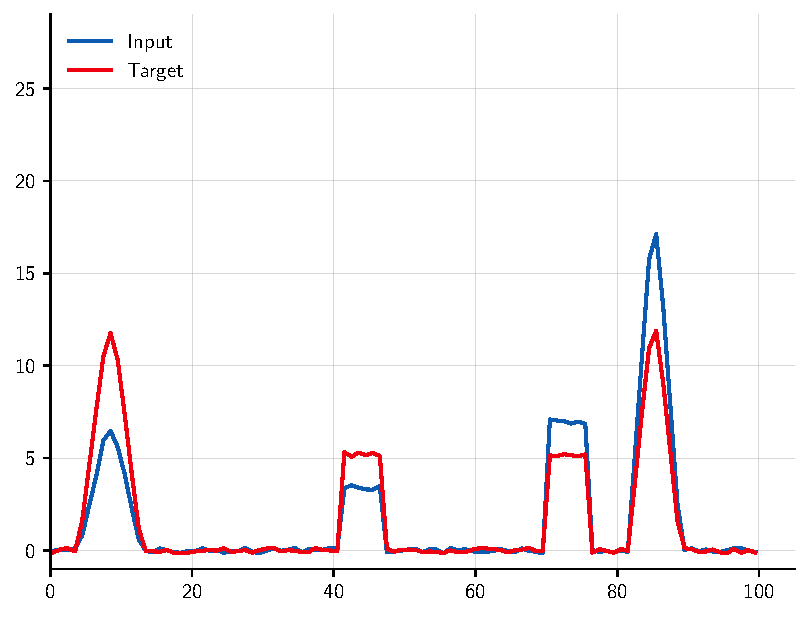
\includegraphics[height=3.50cm]{materials/attention/pics/slides/att1d_train_000.pdf}
%
\hspace{0.5cm}
%
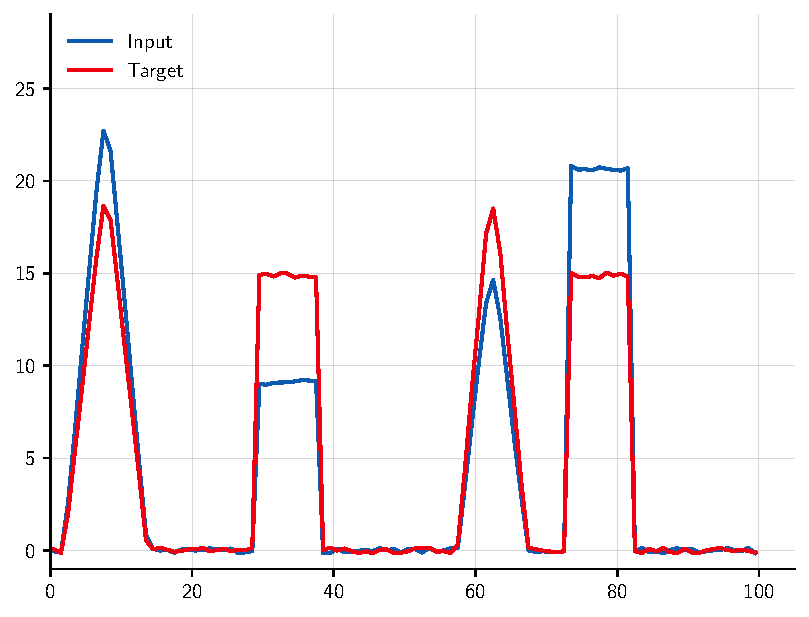
\includegraphics[height=3.50cm]{materials/attention/pics/slides/att1d_train_001.pdf}
}

\makebox[\textwidth][c]{
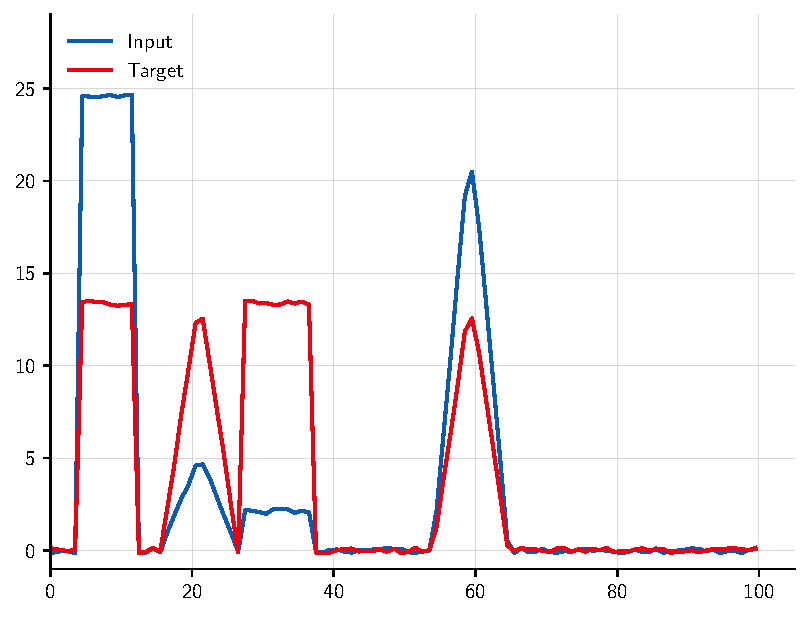
\includegraphics[height=3.50cm]{materials/attention/pics/slides/att1d_train_002.pdf}
%
\hspace{0.5cm}
%
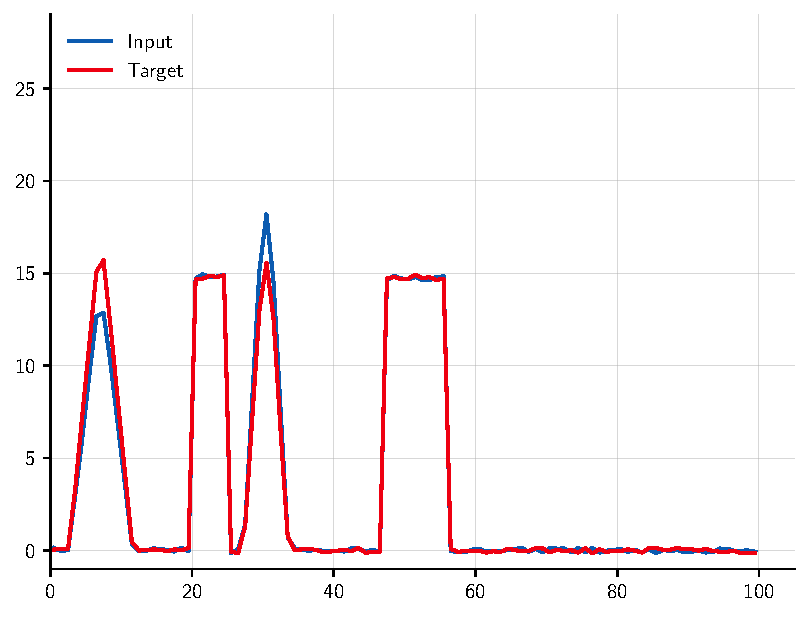
\includegraphics[height=3.50cm]{materials/attention/pics/slides/att1d_train_003.pdf}
}

\end{frame}

%%%%%%%%%%%%%%%%%%%%%%%%%%%%%%%%%%%%%%%%%%%%%%%%%%%%%%%%%%%%%%%%%%%%%%

\begin{frame}[fragile]

We test first a $1$d convolutional network, with no attention
mechanism.

\begin{rawsrc}
Sequential(
  (0): Conv1d(1, 64, kernel_size=(5,), stride=(1,), padding=(2,))
  (1): ReLU()
  (2): Conv1d(64, 64, kernel_size=(5,), stride=(1,), padding=(2,))
  (3): ReLU()
  (4): Conv1d(64, 64, kernel_size=(5,), stride=(1,), padding=(2,))
  (5): ReLU()
  (6): Conv1d(64, 64, kernel_size=(5,), stride=(1,), padding=(2,))
  (7): ReLU()
  (8): Conv1d(64, 1, kernel_size=(5,), stride=(1,), padding=(2,))
)

nb_parameters 62337
\end{rawsrc}

\note[0]{

  As a baseline, we consider a simple convolutional network which
  takes as input the $1$d sequence, procss them with four hidden
  layers with $64$ channels, and outputs a new $1$d sequence.

  Adequate padding preserves the length of the sequence.

}

\end{frame}

%%%%%%%%%%%%%%%%%%%%%%%%%%%%%%%%%%%%%%%%%%%%%%%%%%%%%%%%%%%%%%%%%%%%%%

\begin{frame}[fragile]

Training is done with the MSE loss and Adam.

\rawsrcexcerpt{materials/attention/attentiontoy1d.py}{START_TRAIN}{END_TRAIN}

%% \note[0]{

  %% The MSE loss is used because we want the output sequence to match
  %% the target sequence.

  %% The training procedure is as usual.

%% }

\end{frame}

%%%%%%%%%%%%%%%%%%%%%%%%%%%%%%%%%%%%%%%%%%%%%%%%%%%%%%%%%%%%%%%%%%%%%%

\begin{frame}{}{}

\begin{center}
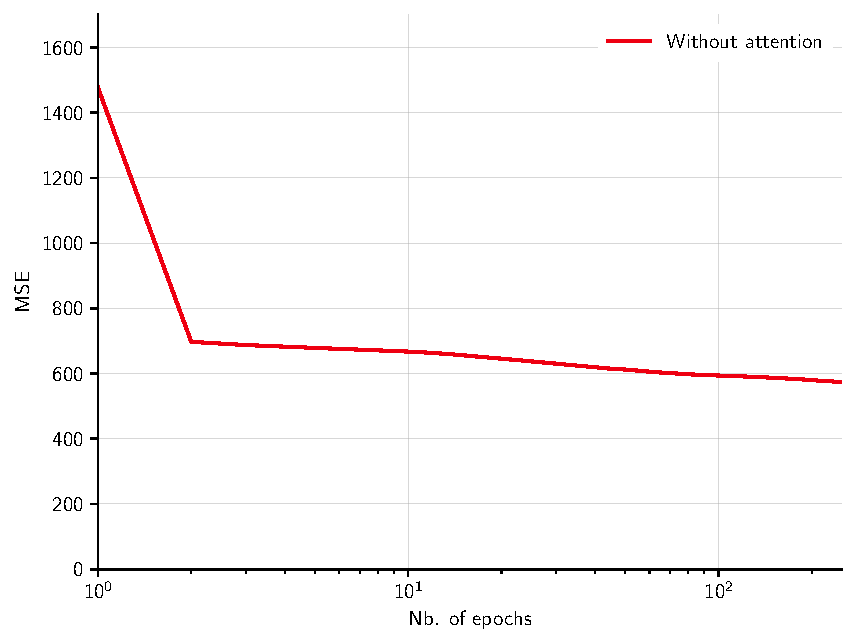
\includegraphics[width=\textwidth]{materials/attention/pics/slides/att1d_train_log.pdf}
\end{center}

\note[0]{

  With such a simple model and no attention, the loss remains
  high. One epoch consists of $25{,}000$ samples.

}

\end{frame}

%%%%%%%%%%%%%%%%%%%%%%%%%%%%%%%%%%%%%%%%%%%%%%%%%%%%%%%%%%%%%%%%%%%%%%

\begin{frame}{}{}

\makebox[\textwidth][c]{
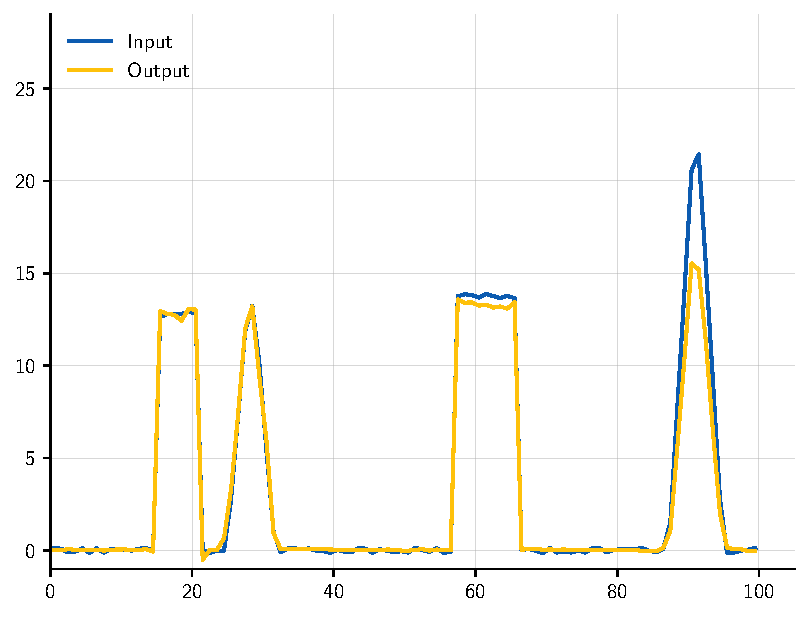
\includegraphics[height=3.50cm]{materials/attention/pics/slides/att1d_test_Y_000.pdf}
%
\hspace{0.5cm}
%
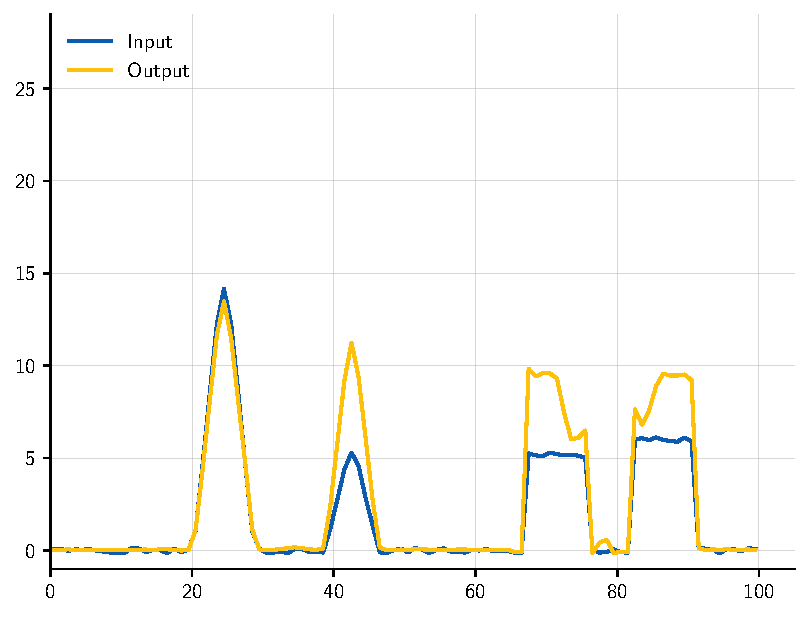
\includegraphics[height=3.50cm]{materials/attention/pics/slides/att1d_test_Y_001.pdf}
}

\makebox[\textwidth][c]{
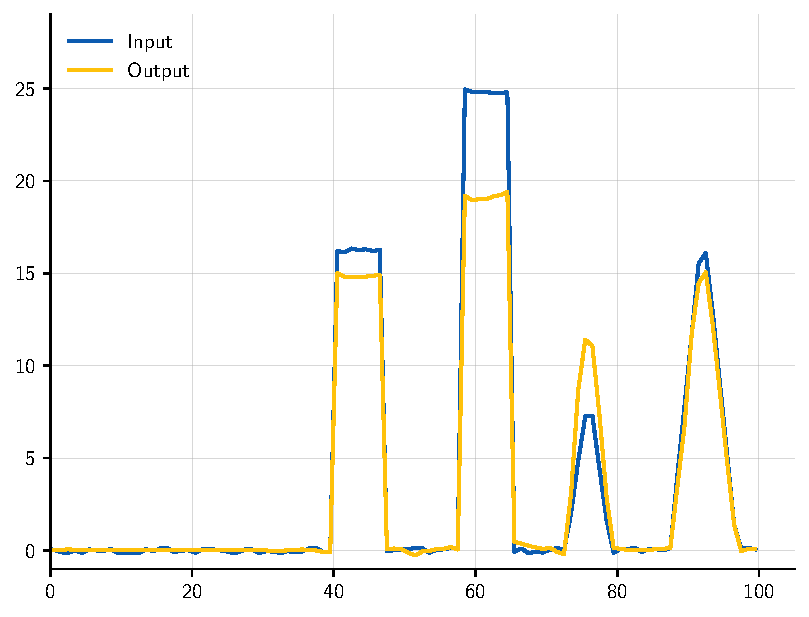
\includegraphics[height=3.50cm]{materials/attention/pics/slides/att1d_test_Y_002.pdf}
%
\hspace{0.5cm}
%
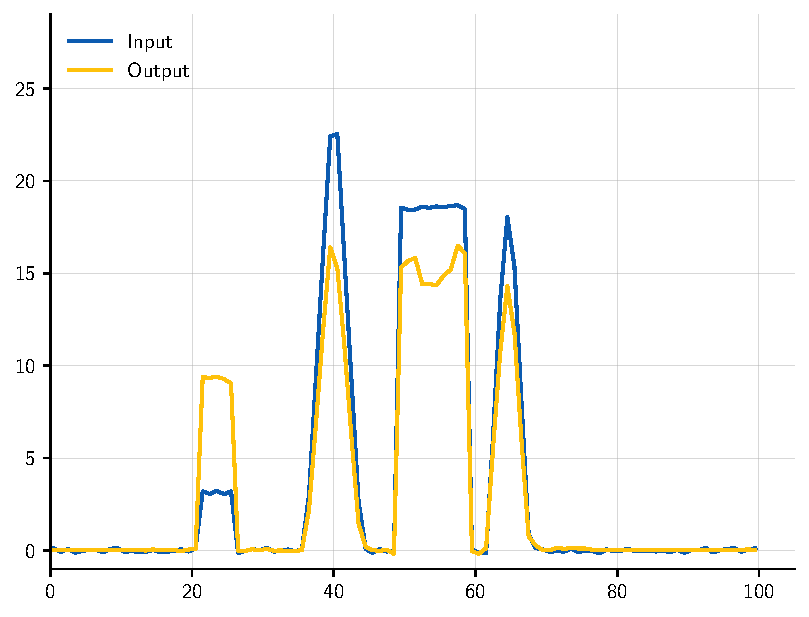
\includegraphics[height=3.50cm]{materials/attention/pics/slides/att1d_test_Y_003.pdf}
}

\note[0]{

  % I don't do specific comment on either of the picture in case they
  % change after regeneration (although seed is put).

  These are example of test results, showing the input in blue, and
  the generated sequences in yellow.

  The output is not that great, which is consistent with the training
  loss remaining high, although we can notice that the model sometimes
  pushes towards the mean when the elements of a pair are close.

}

\end{frame}

%%%%%%%%%%%%%%%%%%%%%%%%%%%%%%%%%%%%%%%%%%%%%%%%%%%%%%%%%%%%%%%%%%%%%%

\begin{frame}{}{}

The poor performance of this model is not surprising given its
inability to transport information from ``far away'' in the
signal. Using more layers, global channel averaging, or fully
connected layers could possibly solve the problem.

However it is more natural to equip the model with the ability to
combine information from parts of the signal that it actively
identifies as relevant.

This is exactly what an attention layer would do.

%% \note[0]{

  %% The main bottleneck of the model is that it is enable to ``look at''
  %% elements far away in the sequence, due to the filter size
  %% of $5$. The receptive field in the input signal of the last units is
  %% not very large.

  %% What we would like to model to do is to detect two patterns of the
  %% same shape, and take their average.

%% }

\end{frame}

%%%%%%%%%%%%%%%%%%%%%%%%%%%%%%%%%%%%%%%%%%%%%%%%%%%%%%%%%%%%%%%%%%%%%%

\begin{frame}{}{}

We implement our own self attention layer with tensors $N \times C
\times T$ so that the products by $W_Q$, $W_K$, and $W_V$
can be implemented as convolutions.

%% To manipulate more clearly the dimensions we use \kw{torch.permute()}
%% that allows to reorder them arbitrarily.

To compute $Q K\transpose$ and $A V$ we need a batch matrix product,
which is provided by \kw{torch.matmul()}.

%% \note[2]{

  %% %% \kw{torch.permute()} allows to reorder the order in which the
  %% %% dimensions of a tensor are visited. For instance, if we have a
  %% %% tensor representing a color image, its size is ${3 \times H \times
    %% %% W}$. To get it in a NumPy fashion, we use

  %% %% % This is ugly, begin{center} adds too much space
  %% %% {\centering \kw{permute(1, 2, 0)},\par}

  %% %% so that
  %% %% \begin{itemize}
  %% %% \item the first dimension of the original tensor ($3$, the number
  %% %% of channels) be in the last position,
  %% %% \item the second dimension of the original tensor (corresponding to
  %% %% the height $H$ of the image) be the first dimension of the output
  %% %% tensor.
  %% %% \end{itemize}
  %% %% The resulting tensor is of size ${H \times W \times 3}$.

  %% As presented in slide \ref{def-matrices-w}, we have
  %% \begin{itemize}
  %% \item a query matrix $Q \in \mathbb{R}^{{T} \times {D}}$,
  %% \item a matrix of keys $K \in \mathbb{R}^{{T'} \times {D}}$,
  %% \item an attention matrix which involves computing $Q \, K\transpose$.
  %% \end{itemize}

  %% \draft{However for efficiency, the input is a batch of $N$ sequences, and
  %% the matrices are actually tensors of shape ${N \times T \times D}$
  %% and ${N \times T' \times D}$. So for each element
  %% ${1 \leq n \leq N}$ of the batch, we want to compute the
  %% corresponding $Q_n \, K_n \transpose$ matrix product, which can be
  %% achieved with \kw{torch.matmul()}.}

%% }

\end{frame}

%%%%%%%%%%%%%%%%%%%%%%%%%%%%%%%%%%%%%%%%%%%%%%%%%%%%%%%%%%%%%%%%%%%%%%

\begin{frame}[fragile]

\begin{comment}
a = torch.rand(11, 9, 2, 3)
b = torch.rand(11, 9, 3, 4)
m = a.matmul(b)
m.size()

m[7, 1]
a[7, 1].mm(b[7, 1])

m[3, 0]
a[3, 0].mm(b[3, 0])
\end{comment}

\begin{rawsrc}
>>> a = torch.rand(11, 9, 2, 3)
>>> b = torch.rand(11, 9, 3, 4)
>>> m = a.matmul(b)
>>> m.size()
torch.Size([11, 9, 2, 4])
>>>
>>> m[7, 1]
tensor([[0.8839, 1.0253, 0.7473, 1.1397],
        [0.4966, 0.5515, 0.4631, 0.6616]])
>>> a[7, 1].mm(b[7, 1])
tensor([[0.8839, 1.0253, 0.7473, 1.1397],
        [0.4966, 0.5515, 0.4631, 0.6616]])
>>>
>>> m[3, 0]
tensor([[0.6906, 0.7657, 0.9310, 0.7547],
        [0.6259, 0.5570, 1.1012, 1.2319]])
>>> a[3, 0].mm(b[3, 0])
tensor([[0.6906, 0.7657, 0.9310, 0.7547],
        [0.6259, 0.5570, 1.1012, 1.2319]])
\end{rawsrc}

\note[0]{

  \kw{a} can be interpreted as a ${11 \times 9}$ matrix of ${2 \times
    3}$ matrices, and \kw{b} as a ${11 \times 9}$ matrix of ${3 \times
    4}$ matrices.

  \kw{matmul} loops over the first dimensions $11 \times 9$ to perform
  every time the product between the matrices of size ${2 \times 3}$
  and ${3 \times 4}$.

  The overall operation results in a ${11 \times 9}$ matrix of $2
  \times 4$ matrices.

}

\end{frame}

%%%%%%%%%%%%%%%%%%%%%%%%%%%%%%%%%%%%%%%%%%%%%%%%%%%%%%%%%%%%%%%%%%%%%%

\begin{frame}[fragile]

%\hspace*{-1cm}
%
\rawsrcexcerpt{materials/attention/attentiontoy1d.py}{START_ATTENTION_LAYER}{END_ATTENTION_LAYER}

\index{attention!layer}

Note that for simplicity it is single-head attention, and the
$1/\sqrt{D}$ is missing.

\pause

The computation of the attention matrix $A$ and the layer's output $Y$
could also be expressed somehow more clearly with Einstein summations
(see lecture \dlcref{einstein-summations}) as

\rawsrcexcerpt{materials/attention/attentiontoy1d.py}{START_EINSTEIN_ATTENTION}{END_EINSTEIN_ATTENTION}[][4]

\note[0]{

  To link between the notations introduced earlier and the current
  implementation, we have:
  %
  \begin{itemize}
  \item $X = X'$ for self attention,
  \item $T = T'$ since the self attention has as many queries as values,
  \item $D = $ \kw{key_dim}, and
  \item $D' = $ \kw{out_dim}.
  \end{itemize}

  The forward function takes as input a batch of size ${N \times C
    \times T}$, so that the products by $W_Q$, $W_K$, and $W_V$ are
  implemented with 1d convolutions. Since the channel comes first per
  sample, to compute the attention matrix ${A = Q K\transpose}$, we
  transpose [the two last dimensions of] $Q$. And similarly to compute
  $A V$, we need to transpose [the two last dimensions of] $V$.

}

\end{frame}

%%%%%%%%%%%%%%%%%%%%%%%%%%%%%%%%%%%%%%%%%%%%%%%%%%%%%%%%%%%%%%%%%%%%%%

\begin{frame}[fragile]

\begin{rawsrc}[commandchars=\\\{\}]
Sequential(
  (0): Conv1d(1, 64, kernel_size=(5,), stride=(1,), padding=(2,))
  (1): ReLU()
  (2): Conv1d(64, 64, kernel_size=(5,), stride=(1,), padding=(2,))
  (3): ReLU()
  (4): SelfAttentionLayer(in_dim=64, out_dim=64, key_dim=64)
  (5): Conv1d(64, 64, kernel_size=(5,), stride=(1,), padding=(2,))
  (6): ReLU()
  (7): Conv1d(64, 1, kernel_size=(5,), stride=(1,), padding=(2,))
)

nb_parameters 54081
\end{rawsrc}

\note[0]{

  We modify our convolutional baseline by replacing the middle
  convolution layer and the following ReLU with the attention layer we
  have implemented.  We choose for the key dimension the same as for
  the values, that is the number of channels.

  Note that the resulting number of parameters is slightly less that
  with the previous convolutional network.

}

\end{frame}

%%%%%%%%%%%%%%%%%%%%%%%%%%%%%%%%%%%%%%%%%%%%%%%%%%%%%%%%%%%%%%%%%%%%%%

\begin{frame}{}{}

\begin{center}
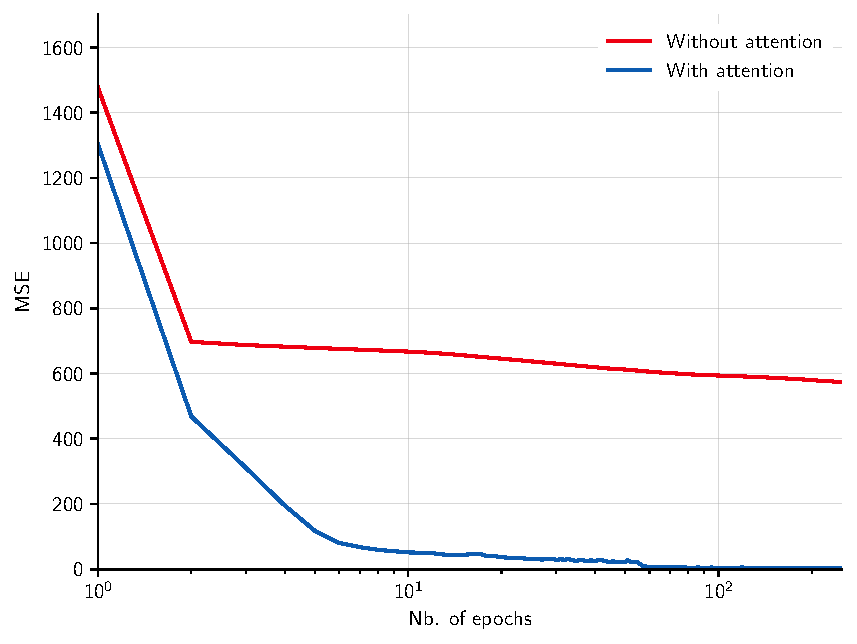
\includegraphics[width=\textwidth]{materials/attention/pics/slides/att1d_wa_train_log.pdf}
\end{center}

\note[0]{

  The exact same training procedure yields much better results with
  the attention layer, as the loss goes down to zero.

}

\end{frame}

%%%%%%%%%%%%%%%%%%%%%%%%%%%%%%%%%%%%%%%%%%%%%%%%%%%%%%%%%%%%%%%%%%%%%%

\begin{frame}{}{}

\makebox[\textwidth][c]{
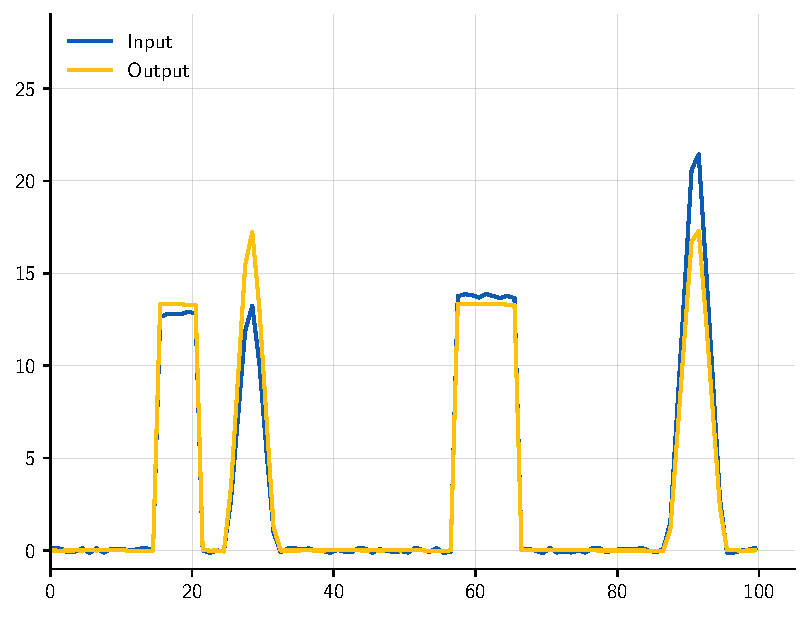
\includegraphics[height=3.50cm]{materials/attention/pics/slides/att1d_wa_test_Y_000.pdf}
%
\hspace{0.5cm}
%
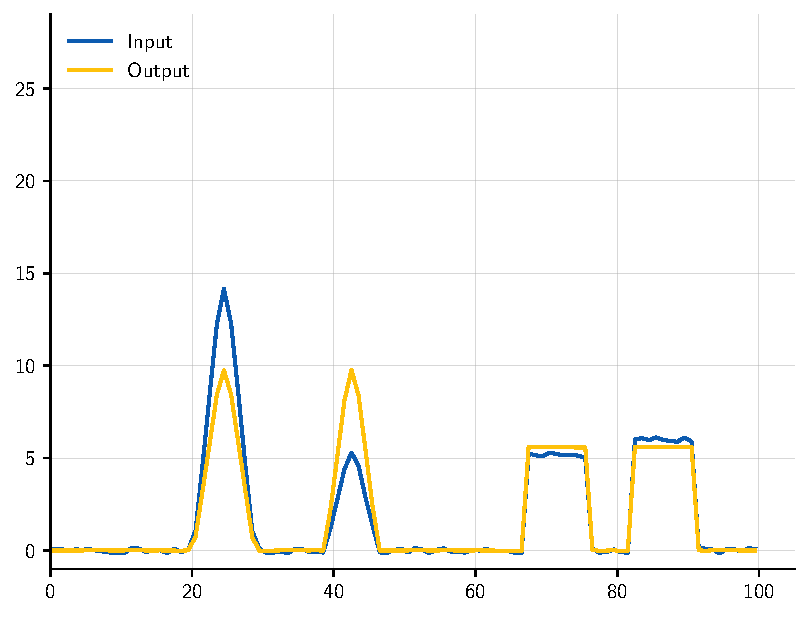
\includegraphics[height=3.50cm]{materials/attention/pics/slides/att1d_wa_test_Y_001.pdf}
}


\makebox[\textwidth][c]{
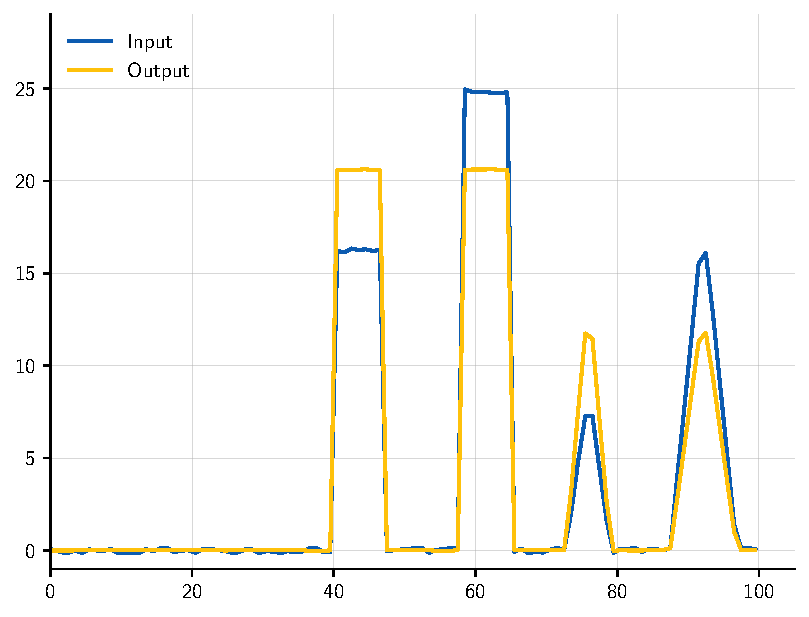
\includegraphics[height=3.50cm]{materials/attention/pics/slides/att1d_wa_test_Y_002.pdf}
%
\hspace{0.5cm}
%
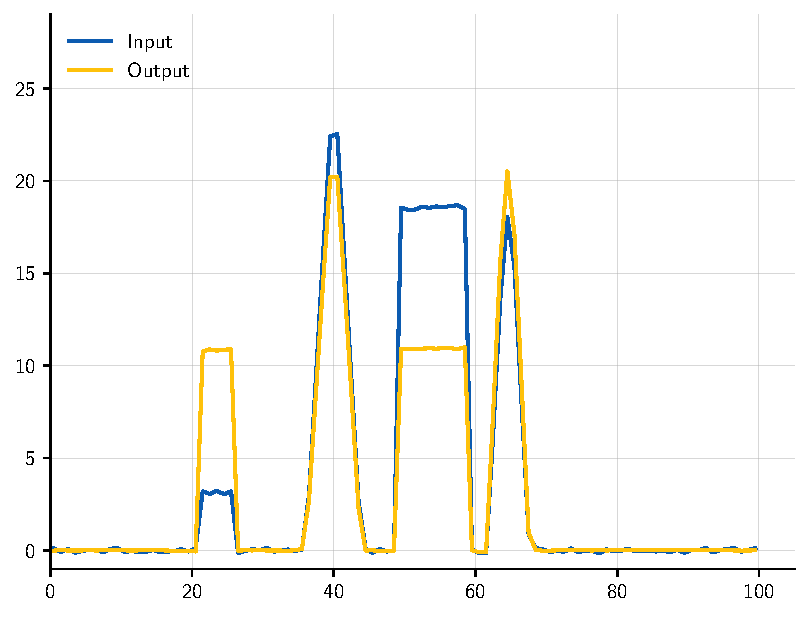
\includegraphics[height=3.50cm]{materials/attention/pics/slides/att1d_wa_test_Y_003.pdf}
}

\note[0]{

  These are example results obtained with the attention network,
  showing the input in blue, and the generated sequences in yellow.

  The network does what is it supposed to do. We can see that the
  height of each pair is now averaged properly.

}

\end{frame}

%%%%%%%%%%%%%%%%%%%%%%%%%%%%%%%%%%%%%%%%%%%%%%%%%%%%%%%%%%%%%%%%%%%%%%

\begin{frame}{}{}

\only<+>{
\makebox[\textwidth][c]{
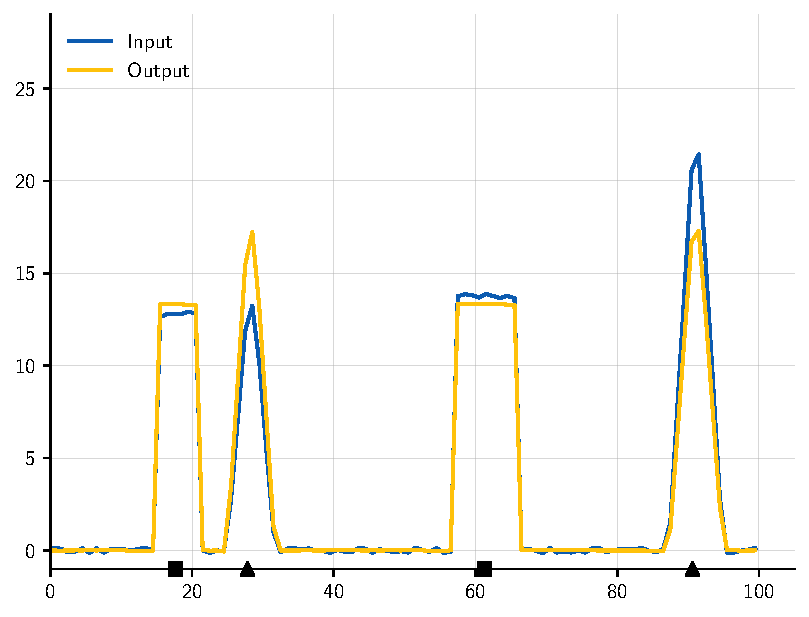
\includegraphics[height=3.50cm]{materials/attention/pics/slides/att1d_wa_test_Yp_000.pdf}
%
\hspace*{0.5cm}
%
\raisebox{-0.25cm}{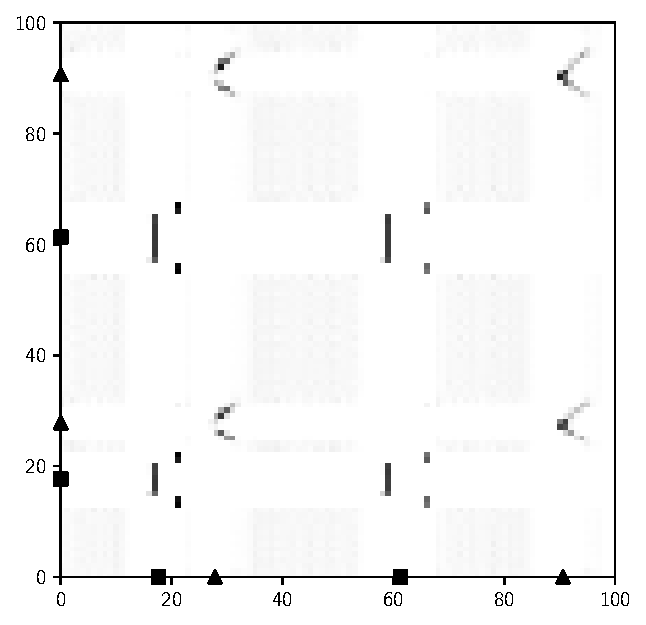
\includegraphics[height=4.00cm]{materials/attention/pics/slides/att1d_wa_test_A_000.pdf}}
}}

\only<+>{
\makebox[\textwidth][c]{
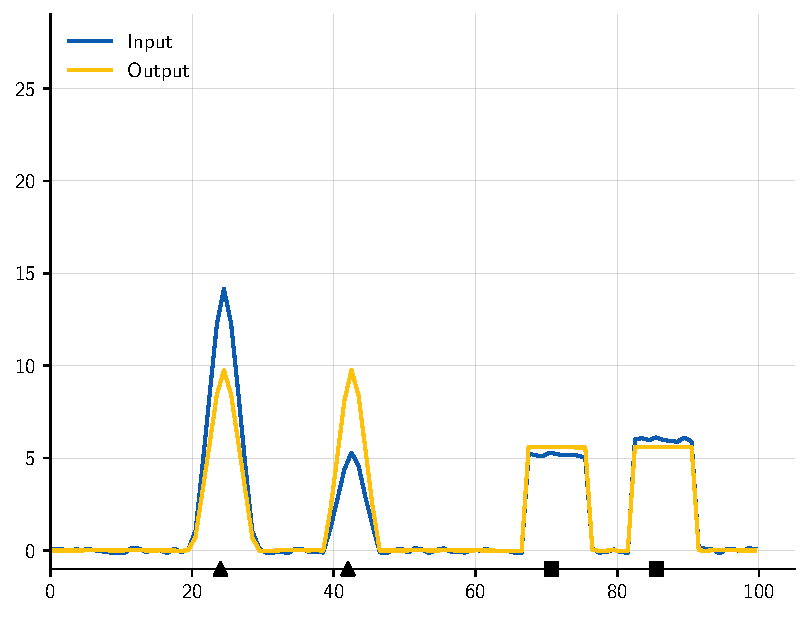
\includegraphics[height=3.50cm]{materials/attention/pics/slides/att1d_wa_test_Yp_001.pdf}
%
\hspace*{0.5cm}
%
\raisebox{-0.25cm}{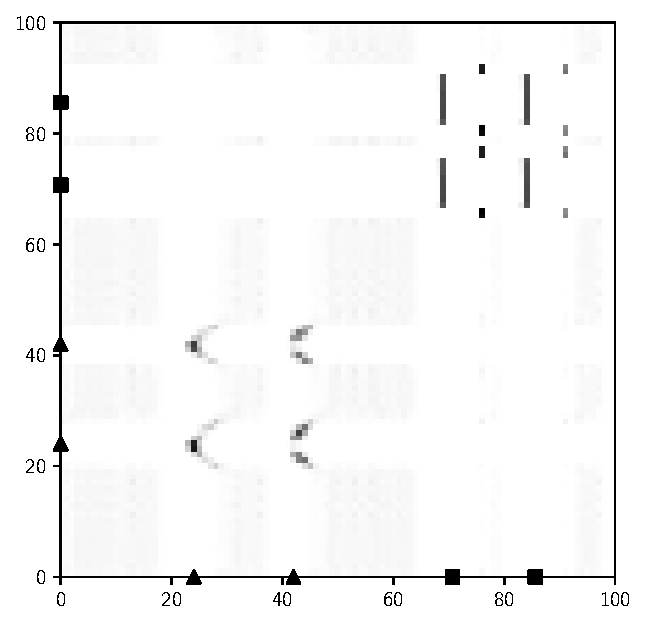
\includegraphics[height=4.00cm]{materials/attention/pics/slides/att1d_wa_test_A_001.pdf}}
}}

\mode<beamer>{\only<+>{
\makebox[\textwidth][c]{
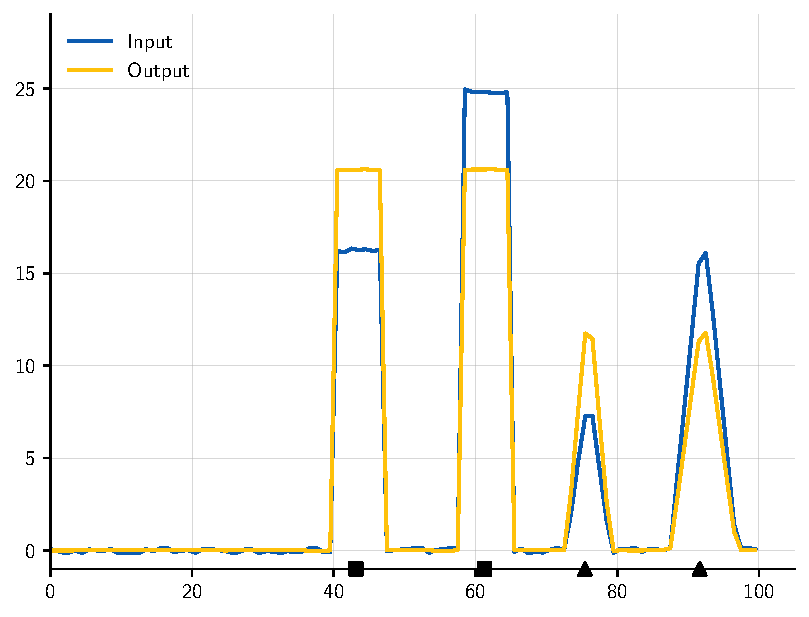
\includegraphics[height=3.50cm]{materials/attention/pics/slides/att1d_wa_test_Yp_002.pdf}
%
\hspace*{0.5cm}
%
\raisebox{-0.25cm}{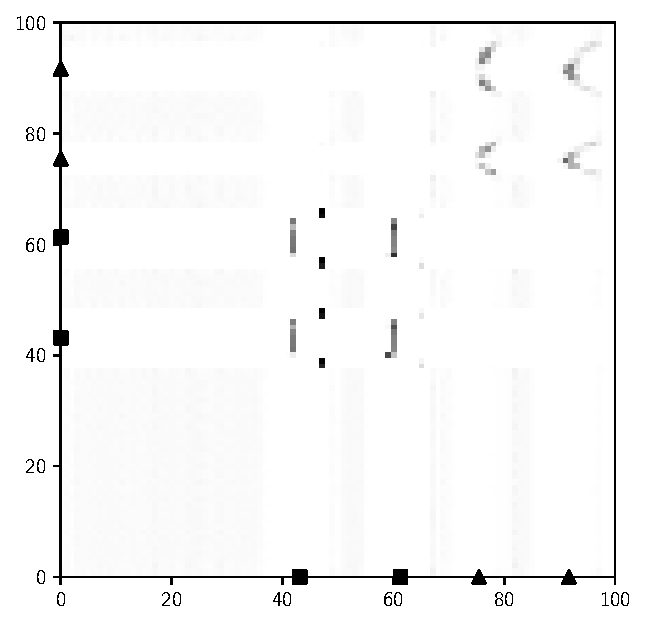
\includegraphics[height=4.00cm]{materials/attention/pics/slides/att1d_wa_test_A_002.pdf}}
}}}

\note[0]{

  The images on the left are test sequences. Markers are placed at the
  indexes of the sequence corresponding to the shape centers: black
  squares for the rectangles, and black triangles for triangles.

  The images on the right are the attention matrices, with white
  standing for small coefficients and black for large ones.

  This shows that each pair of shapes attend at each other. Rectangles
  put attention on the boundary of their edges, and the triangles put
  emphasis on their respective slopes.

}

\end{frame}

%%%%%%%%%%%%%%%%%%%%%%%%%%%%%%%%%%%%%%%%%%%%%%%%%%%%%%%%%%%%%%%%%%%%%%

\begin{frame}

\begin{warning}
Because it is invariant to a permutation of the keys and values, such
an attention layer disregards the absolute location of the values.
\end{warning}

%% \vspace*{2ex}

%% Given any permutation
%% %
%% \[
%% \sigma: \{ 1, \dots, S \} \rightarrow \{ 1, \dots, S \},
%% \]
%% %
%% we have
%% %
%% \[
%% Y_{j} = \sum_i \softmax_i \left( Q_{j} K_{\sigma(i)}\transpose \right) V_{\sigma(i)}.
%% \]

%% %% \[
%% %% %% {Y}_{j} = \sum_{i=1}^{T} \softmax_i \left(a\left({C}_{j}, {V}_{\xi(i)}; \theta\right)\right) {V}_{\xi(i)}.
%% %% \]

%% \pause

%% The formal definition of this operation does not require any ordering
%% property on the indexing of the key/values.

 %% %% The only thing is that, except for
%% %% the final dimension, ${Y}$ has the same shape as ${Q}$.

%% %% \note[0]{

  %% %% One major drawback of the attention mechanism presented is that
  %% %% should a permutation $\sigma_i$ be applied consistently on both the
  %% %% values and the keys, the output $Y_j$ would be unchanged.

%% %% }

%% \end{frame}

%% %%%%%%%%%%%%%%%%%%%%%%%%%%%%%%%%%%%%%%%%%%%%%%%%%%%%%%%%%%%%%%%%%%%%%%

%% \begin{frame}{}{}

Our toy problem does not require to take into account the positioning
in the tensor. We can modify it with a target where the pairs to
average are the two rightmost and leftmost shapes.

\vspace*{4ex}

\makebox[\textwidth][c]{
\uncover<2-5>{
\begin{tikzpicture}[scale=0.45]

  \colorlet{groupAinput}{blue}
  \colorlet{groupBinput}{blue}
  \colorlet{groupAtarget}{darkred}
  \colorlet{groupBtarget}{darkred}

  \mode<beamer>{
    \only<beamer:3>{%
      \colorlet{groupAinput}{blue}
      \colorlet{groupBinput}{blue!15}
      \colorlet{groupAtarget}{darkred}
      \colorlet{groupBtarget}{darkred!15}
    }

    \only<beamer:4>{%
      \colorlet{groupAinput}{blue!15}
      \colorlet{groupBinput}{blue}
      \colorlet{groupAtarget}{darkred!15}
      \colorlet{groupBtarget}{darkred}
    }
  }

  \draw[color=groupAinput,thick] (0.5, 0) -- ++(1.1, 2.0) -- ++(1.1, -2);
  \draw[color=groupAinput,thick] (3.2, 0) -- ++(0.0, 0.5) -- ++(1.2, 0.0) -- ++(0.0, -0.5);
  \draw[color=groupBinput,thick] (5.5, 0) -- ++(0.0, 3.5) -- ++(0.8, 0.0) -- ++(0.0, -3.5);
  \draw[color=groupBinput,thick] (8.5, 0) -- ++(0.6, 6.0) -- ++(0.6, -6);

  \draw[black] ( 0.0, -0.25) -- ++(0.0, 6.5);
  \draw[black] (10.0, -0.25) -- ++(0.0, 6.5);
  \draw[black] (-0.25, -0.00) -- ++(10.5, -0.0) node[midway,below,yshift=-1mm] {Input};

  %----------

  \begin{scope}[shift={(13, 0.0)}]
    \draw[color=groupAtarget,thick] (0.5, 0) -- ++(1.1, 1.25) -- ++(1.1, -1.25);
    \draw[color=groupAtarget,thick] (3.2, 0) -- ++(0.0, 1.25) -- ++(1.2, 0.0) -- ++(0.0, -1.25);
    \draw[color=groupBtarget,thick] (5.5, 0) -- ++(0.0, 4.75) -- ++(0.8, 0.0) -- ++(0.0, -4.75);
    \draw[color=groupBtarget,thick] (8.5, 0) -- ++(0.6, 4.75) -- ++(0.6, -4.75);

    \draw[black] ( 0.0, -0.25) -- ++(0.0, 6.5);
    \draw[black] (10.0, -0.25) -- ++(0.0, 6.5);
    \draw[black] (-0.25, -0.00) -- ++(10.5, -0.0) node[midway,below,yshift=-1mm] {Target};
  \end{scope};

  %---------

  \mode<beamer>{
    \uncover<3>{\scalelines{1.5}{2.0}{3.2}{0.5}{17.4}{1.25}}
    \uncover<4>{\scalelines{5.5}{3.5}{8.5}{6.0}{23.0}{4.75}}
  }

  \mode<handout>{
    \draw[draw=none] (1.6, 3.5) -- (3.8, 3.5) node[midway,above,gray,yshift=-1pt,font=\footnotesize] {leftmost};
    \draw[gray,{Bar[width=1.5mm]}-,shorten <= 1.5pt] ($(0.5, 2.0)+(1.1, 0)$) |- (2.35, 3.5);
    \draw[gray,{Bar[width=1.5mm]}-,shorten <= 1.5pt] ($(3.2, 0.5)+(0.6, 0)$) |- (2.35, 3.5);
    \begin{scope}[shift={(13, 0.0)}]
      \draw[draw=none] (1.6, 3.5) -- (3.8, 3.5) node[midway,above,gray,yshift=-1pt,font=\footnotesize] {leftmost};
      \draw[gray,{Bar[width=1.5mm]}-,shorten <= 1.5pt] ($(0.5, 1.25)+(1.1, 0)$) |- (2.35, 3.5);
      \draw[gray,{Bar[width=1.5mm]}-,shorten <= 1.5pt] ($(3.2, 1.25)+(0.6, 0)$) |- (2.35, 3.5);
    \end{scope}

    \draw[draw=none] (5.9, 6.5) -- (9.1, 6.5) node[midway,above,gray,yshift=-1pt,font=\footnotesize] {rightmost};
    \draw[gray,{Bar[width=1.5mm]}-,shorten <= 1.5pt] ($(5.5, 3.5)+(0.4, 0)$) |- (7.00, 6.5);
    \draw[gray,{Bar[width=1.5mm]}-,shorten <= 1.5pt] ($(8.5, 6.0)+(0.6, 0)$) |- (7.00, 6.5);
    \begin{scope}[shift={(13, 0.0)}]
      \draw[draw=none] (5.9, 6.5) -- (9.1, 6.5) node[midway,above,gray,yshift=-1pt,font=\footnotesize] {rightmost};
      \draw[gray,{Bar[width=1.5mm]}-,shorten <= 1.5pt] ($(5.5, 4.75)+(0.4, 0)$) |- (7.00, 6.5);
      \draw[gray,{Bar[width=1.5mm]}-,shorten <= 1.5pt] ($(8.5, 4.75)+(0.6, 0)$) |- (7.00, 6.5);
    \end{scope}
  }

\end{tikzpicture}
}
}

\note[0]{

  To illustrate this drawback, we design a new synthetic task in which
  the goal is to average the heights of the two leftmost shapes with
  each other, and the heights of the two rightmost with each other.

  Such a task still requires attention, because it involves
  looking at features far away from one another, but be able to take
  into account locations.

}

\end{frame}

%%%%%%%%%%%%%%%%%%%%%%%%%%%%%%%%%%%%%%%%%%%%%%%%%%%%%%%%%%%%%%%%%%%%%%

\begin{frame}{}{}

Some training examples.

\vspace*{-1.5ex}

\makebox[\textwidth][c]{
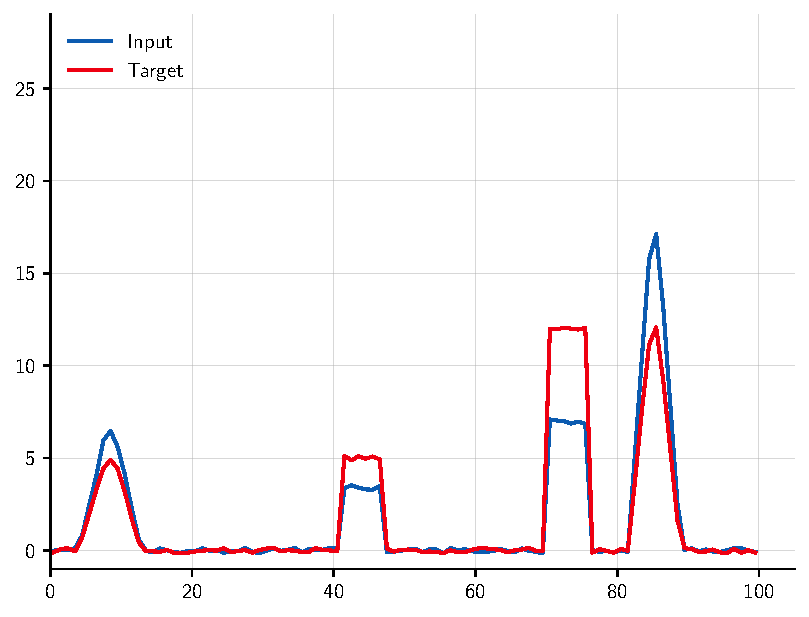
\includegraphics[height=3.50cm]{materials/attention/pics/slides/att1d_wa_lg_train_000.pdf}
%
\hspace{0.5cm}
%
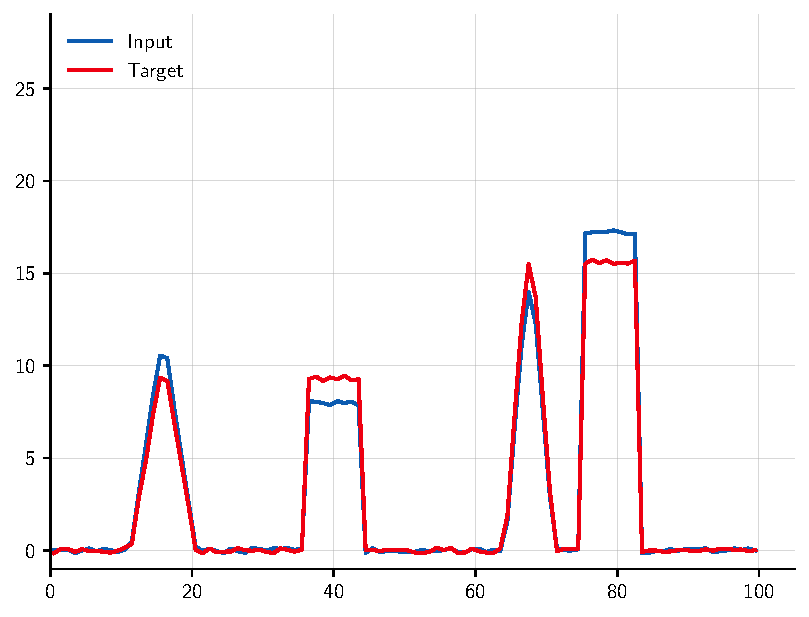
\includegraphics[height=3.50cm]{materials/attention/pics/slides/att1d_wa_lg_train_001.pdf}
}

\makebox[\textwidth][c]{
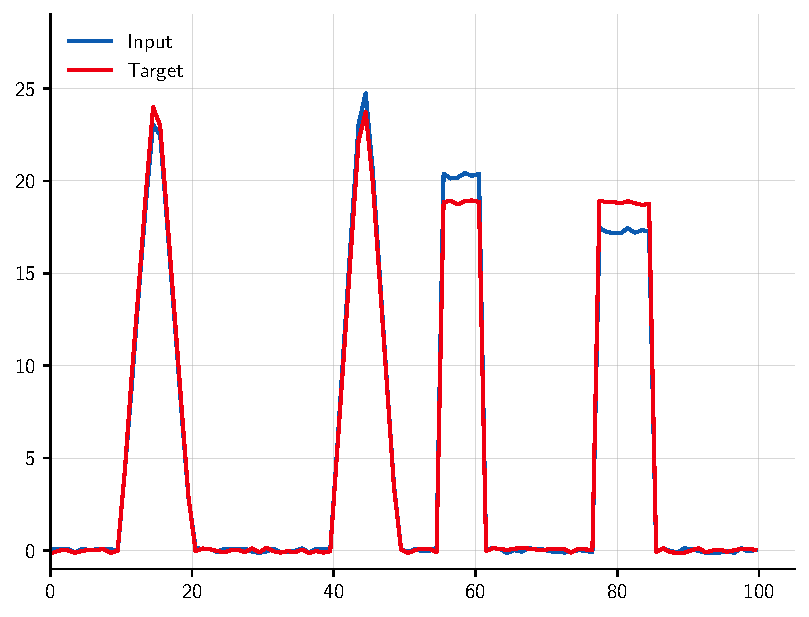
\includegraphics[height=3.50cm]{materials/attention/pics/slides/att1d_wa_lg_train_002.pdf}
%
\hspace{0.5cm}
%
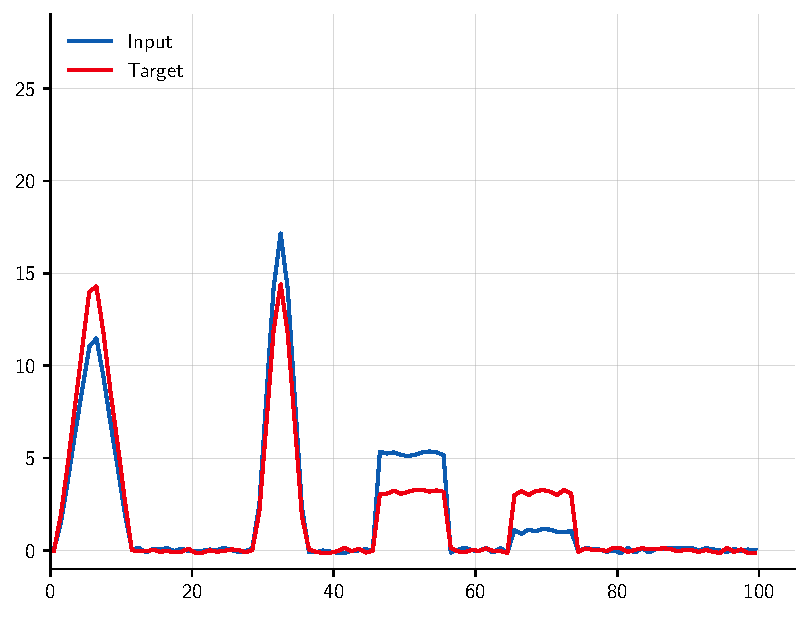
\includegraphics[height=3.50cm]{materials/attention/pics/slides/att1d_wa_lg_train_003.pdf}
}

%% \note[0]{

  %% These training examples illustrate that the task is to average the
  %% height of the first two shapes, and the height of the last two ones.

%% }

\end{frame}

%%%%%%%%%%%%%%%%%%%%%%%%%%%%%%%%%%%%%%%%%%%%%%%%%%%%%%%%%%%%%%%%%%%%%%

\begin{frame}{}{}

\begin{center}
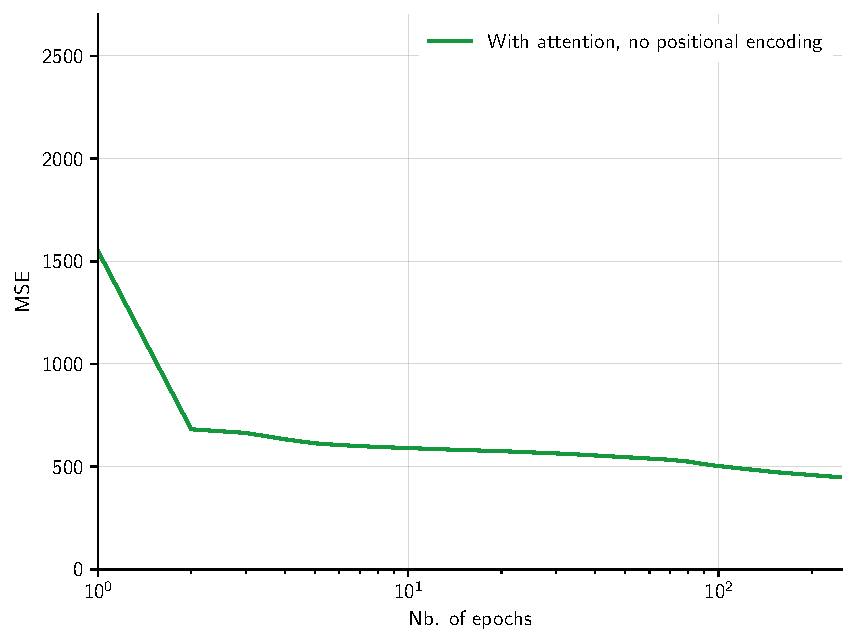
\includegraphics[width=\textwidth]{materials/attention/pics/slides/att1d_wa_lg_train_log.pdf}
\end{center}

\note[0]{

  Our attention model on this new task performs almost as badly as the
  convolutional network on the first task.

}

\end{frame}

%%%%%%%%%%%%%%%%%%%%%%%%%%%%%%%%%%%%%%%%%%%%%%%%%%%%%%%%%%%%%%%%%%%%%%

\begin{frame}{}{}

\makebox[\textwidth][c]{
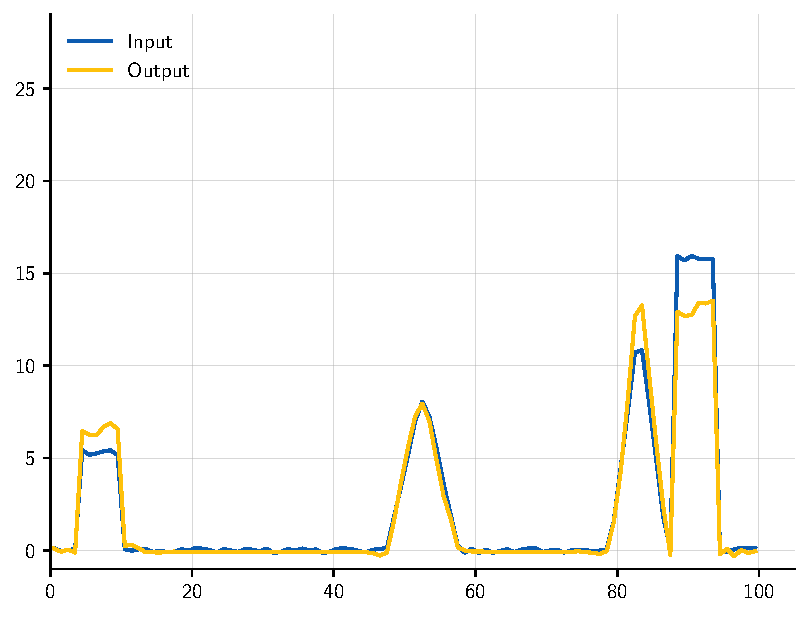
\includegraphics[height=3.50cm]{materials/attention/pics/slides/att1d_wa_lg_test_Y_000.pdf}
%
\hspace{0.5cm}
%
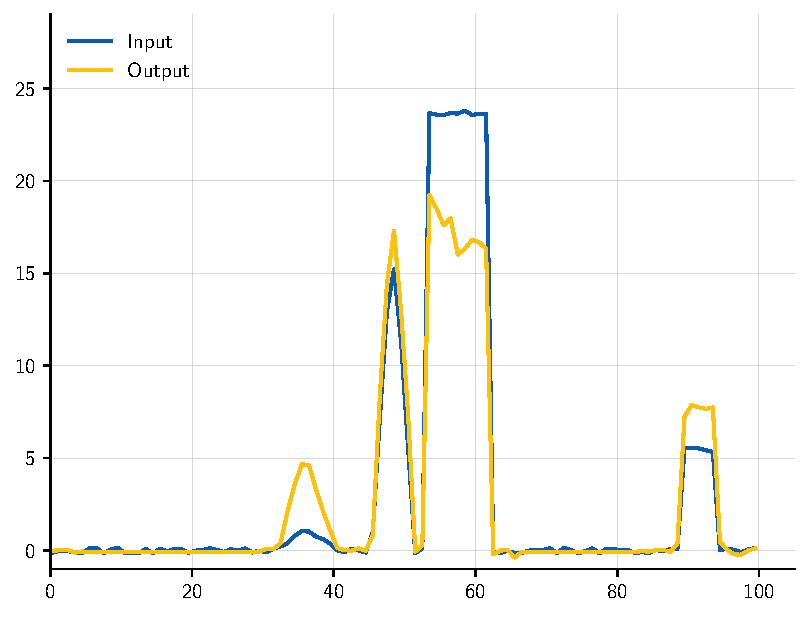
\includegraphics[height=3.50cm]{materials/attention/pics/slides/att1d_wa_lg_test_Y_001.pdf}
}

\makebox[\textwidth][c]{
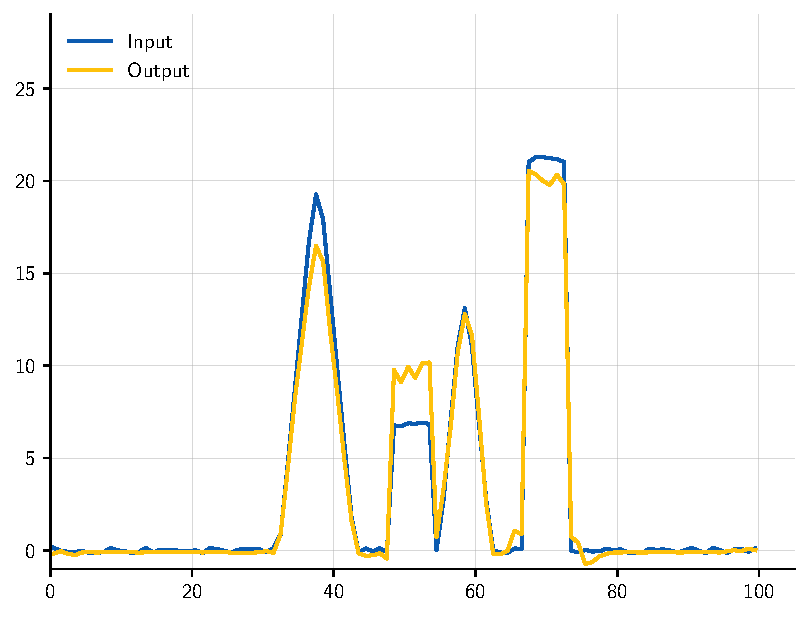
\includegraphics[height=3.50cm]{materials/attention/pics/slides/att1d_wa_lg_test_Y_002.pdf}
%
\hspace{0.5cm}
%
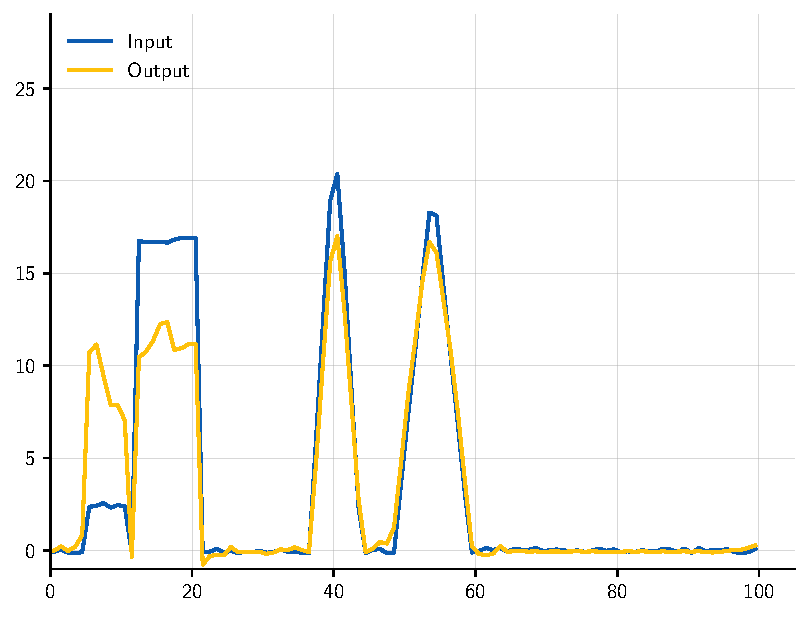
\includegraphics[height=3.50cm]{materials/attention/pics/slides/att1d_wa_lg_test_Y_003.pdf}
}

%% \note[0]{

  %% These plots are the results of the original attention model.

  %% \draft{These results are not that bad...}

%% }

\end{frame}

%%%%%%%%%%%%%%%%%%%%%%%%%%%%%%%%%%%%%%%%%%%%%%%%%%%%%%%%%%%%%%%%%%%%%%

\begin{frame}[fragile]

The poor performance of this model is not surprising given its
inability to take into account positions in the attention layer.

We can fix this by providing to the model a \textbf{positional
  encoding}\index{positional encoding}.

\begin{comment}
slen = 20
c = math.ceil(math.log(len) / math.log(2.0))
o = 2**torch.arange(c).unsqueeze(1)
pe = (torch.arange(len).unsqueeze(0).div(o, rounding_mode = 'floor')) % 2
pe
input = torch.rand(5, 3, len)
pe = pe[None].float()
input = torch.cat((input, pe.expand(input.size(0), -1, -1)), 1)
\end{comment}

\begin{rawsrc}
>>> len = 20
>>> c = math.ceil(math.log(len) / math.log(2.0))
>>> o = 2**torch.arange(c).unsqueeze(1)
>>> pe = (torch.arange(len).unsqueeze(0).div(o, rounding_mode = 'floor')) % 2
>>> pe
tensor([[0, 1, 0, 1, 0, 1, 0, 1, 0, 1, 0, 1, 0, 1, 0, 1, 0, 1, 0, 1],
        [0, 0, 1, 1, 0, 0, 1, 1, 0, 0, 1, 1, 0, 0, 1, 1, 0, 0, 1, 1],
        [0, 0, 0, 0, 1, 1, 1, 1, 0, 0, 0, 0, 1, 1, 1, 1, 0, 0, 0, 0],
        [0, 0, 0, 0, 0, 0, 0, 0, 1, 1, 1, 1, 1, 1, 1, 1, 0, 0, 0, 0],
        [0, 0, 0, 0, 0, 0, 0, 0, 0, 0, 0, 0, 0, 0, 0, 0, 1, 1, 1, 1]])
\end{rawsrc}

Such a tensor can simply be channel-concatenated to the input batch:

\begin{rawsrc}
>>> pe = pe[None].float()
>>> input = torch.cat((input, pe.expand(input.size(0), -1, -1)), 1)
\end{rawsrc}

\note[0]{

  The positional encoding aims at augmenting the input tensor with a
  binary code which completely determines the location in the
  sequence. With a sequence of length $20$, $B=5$ channels suffice:
  the first element is associated to code ${(0, 0, 0, 0, 0)}$, the
  second to ${(0, 0, 0, 0, 1)}$, {etc.} which are the binary encoding
  of the index.

  A minibatch of $N$ samples representing sequences of $T$ elements of
  dimension $D$, is of size ${N \times D \times T}$. After the
  positional encoding is concatenated as channels to the dimension of
  the elements, the minibatch is of shape ${N \times (D + B) \times
    T}$.

  Other coding scheme exists, for instance using trigonometric
  functions instead of a hard binary encoding.

}

\end{frame}

%%%%%%%%%%%%%%%%%%%%%%%%%%%%%%%%%%%%%%%%%%%%%%%%%%%%%%%%%%%%%%%%%%%%%%

\begin{frame}{}{}

\begin{center}
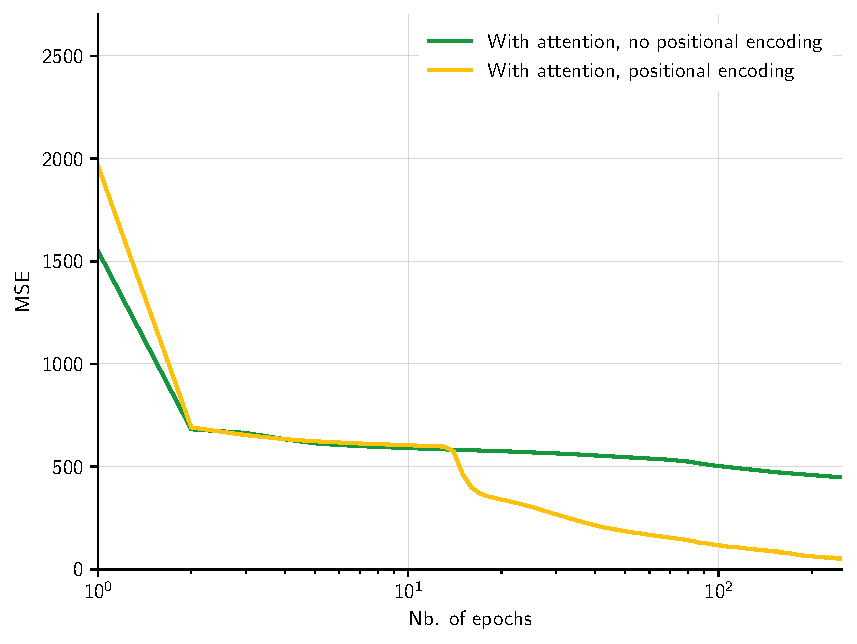
\includegraphics[width=\textwidth]{materials/attention/pics/slides/att1d_wa_lg_pe_train_log.pdf}
\end{center}

\note[0]{

  The graph shows the training losses of our attention model with and
  without positional encoding.

}

\end{frame}

%%%%%%%%%%%%%%%%%%%%%%%%%%%%%%%%%%%%%%%%%%%%%%%%%%%%%%%%%%%%%%%%%%%%%%

\begin{frame}{}{}

\makebox[\textwidth][c]{
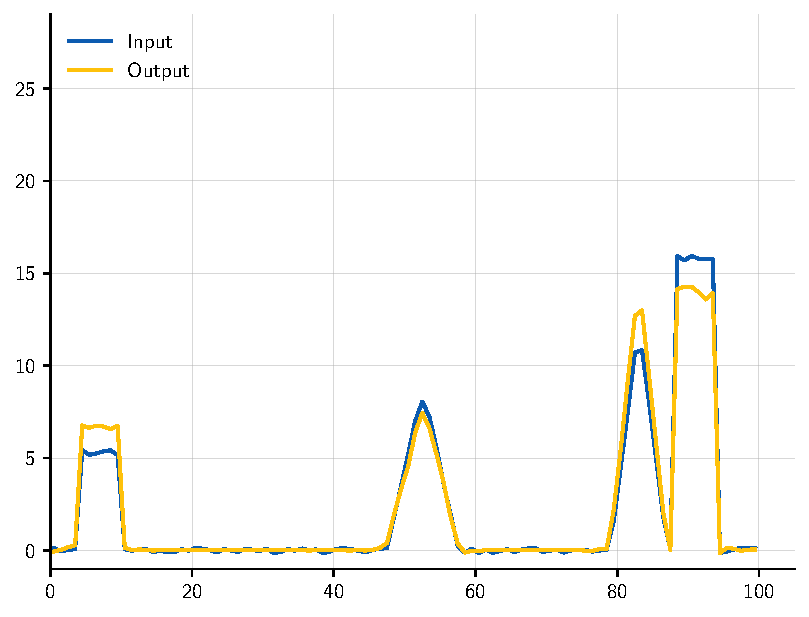
\includegraphics[height=3.50cm]{materials/attention/pics/slides/att1d_wa_lg_pe_test_Y_000.pdf}
%
\hspace{0.5cm}
%
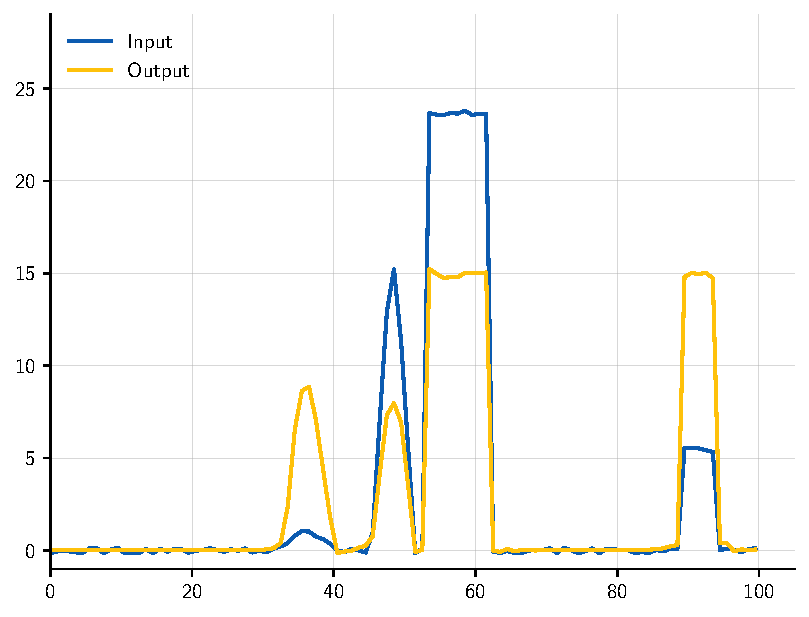
\includegraphics[height=3.50cm]{materials/attention/pics/slides/att1d_wa_lg_pe_test_Y_001.pdf}
}


\makebox[\textwidth][c]{
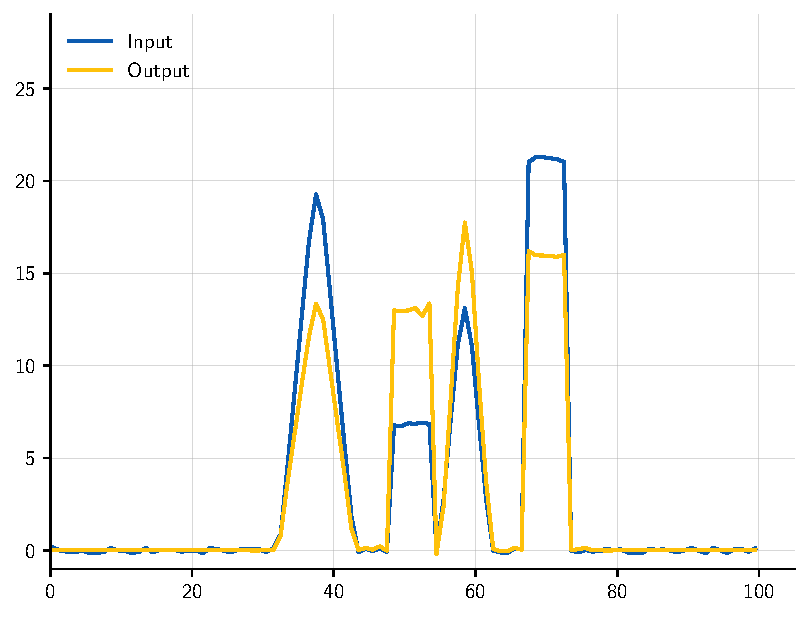
\includegraphics[height=3.50cm]{materials/attention/pics/slides/att1d_wa_lg_pe_test_Y_002.pdf}
%
\hspace{0.5cm}
%
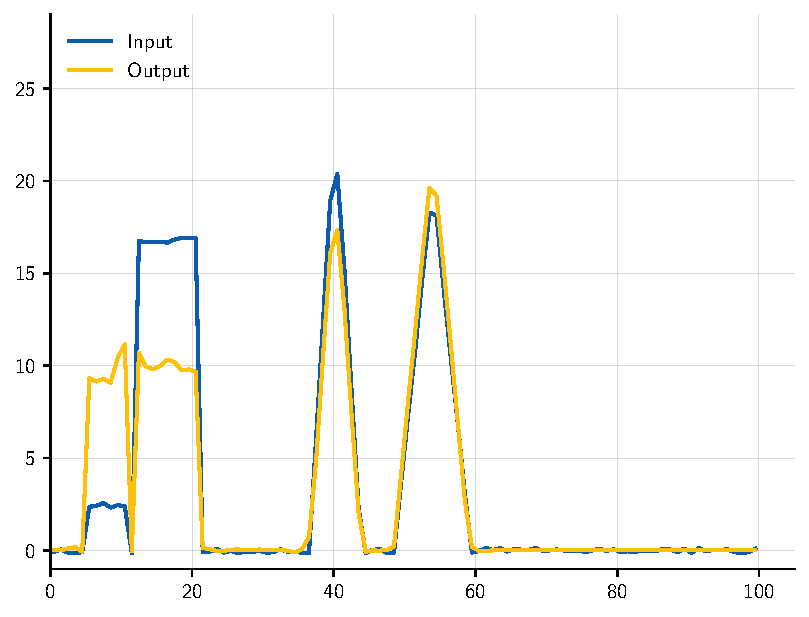
\includegraphics[height=3.50cm]{materials/attention/pics/slides/att1d_wa_lg_pe_test_Y_003.pdf}
}

\end{frame}

%%%%%%%%%%%%%%%%%%%%%%%%%%%%%%%%%%%%%%%%%%%%%%%%%%%%%%%%%%%%%%%%%%%%%%

\begin{frame}{}{}

\only<+>{
\makebox[\textwidth][c]{
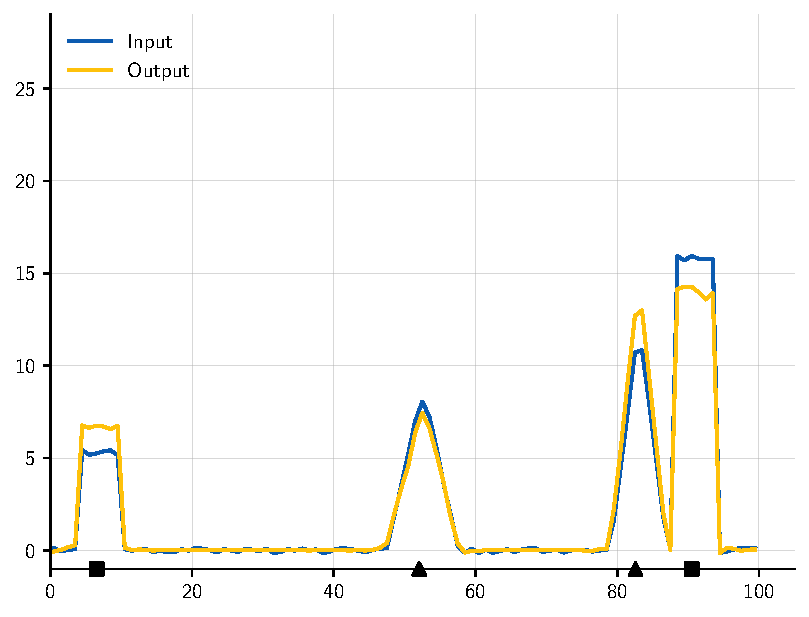
\includegraphics[height=3.50cm]{materials/attention/pics/slides/att1d_wa_lg_pe_test_Yp_000.pdf}
%
\hspace*{0.5cm}
%
\raisebox{-0.25cm}{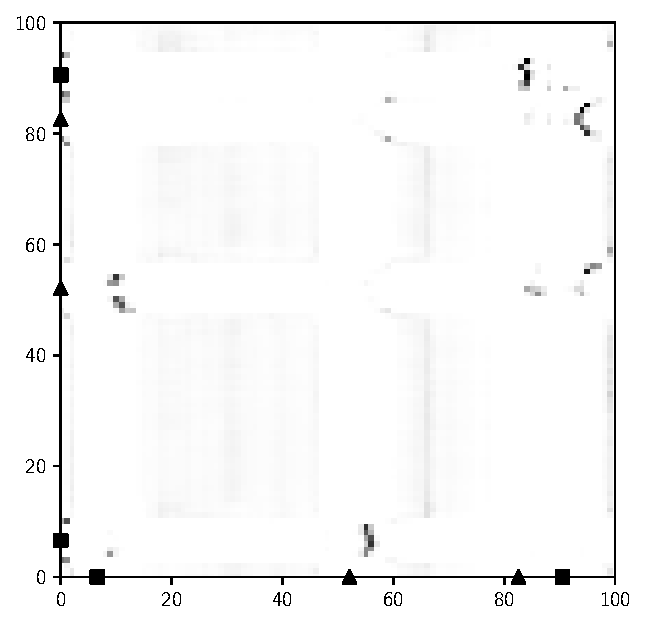
\includegraphics[height=4.00cm]{materials/attention/pics/slides/att1d_wa_lg_pe_test_A_000.pdf}}
}}

\only<+>{
\makebox[\textwidth][c]{
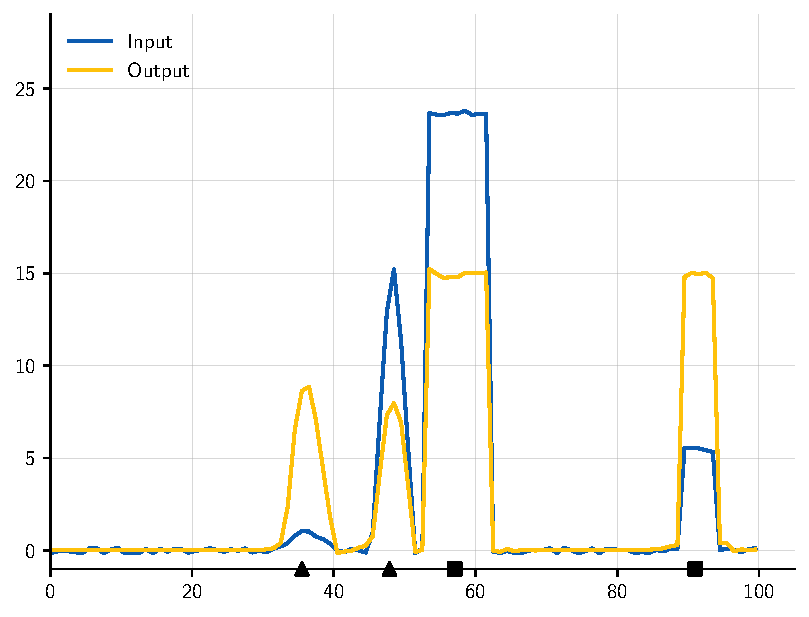
\includegraphics[height=3.50cm]{materials/attention/pics/slides/att1d_wa_lg_pe_test_Yp_001.pdf}
%
\hspace*{0.5cm}
%
\raisebox{-0.25cm}{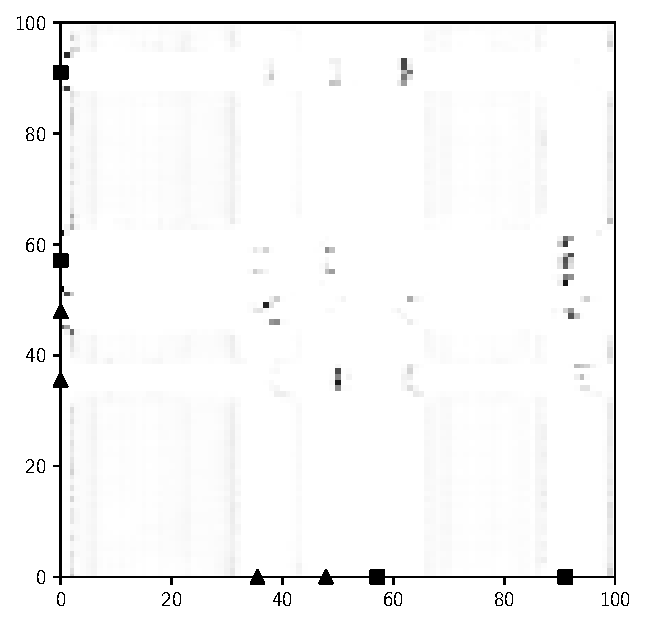
\includegraphics[height=4.00cm]{materials/attention/pics/slides/att1d_wa_lg_pe_test_A_001.pdf}}
}}

\mode<beamer>{\only<+>{
\makebox[\textwidth][c]{
\includegraphics[height=3.50cm]{materials/attention/pics/slides/att1d_wa_lg_pe_test_Yp_002.pdf}
%
\hspace*{0.5cm}
%
\raisebox{-0.25cm}{\includegraphics[height=4.00cm]{materials/attention/pics/slides/att1d_wa_lg_pe_test_A_002.pdf}}
}}}


\note[0]{

  The images on the left are test sequences. Markers are placed at the
  indexes of the sequence corresponding to the shape centers: black
  squares for the rectangles, and black triangles for triangles.

  The images on the right are the attention matrices, with white
  standing for small coefficients and black for large ones.

  Although not as strong as in the previous task, we can see that the
  attention is put on the first two shapes jointly, and on the last
  two jointly.

}

\end{frame}

%%%%%%%%%%%%%%%%%%%%%%%%%%%%%%%%%%%%%%%%%%%%%%%%%%%%%%%%%%%%%%%%%%%%%%

\closingframe

\bibliographyframe

%%%%%%%%%%%%%%%%%%%%%%%%%%%%%%%%%%%%%%%%%%%%%%%%%%%%%%%%%%%%%%%%%%%%%%

\checknbdrafts

\end{document}
